\documentclass[a4paper, 11pt,oneside,openany, danish]{memoir} % Starter dokumentet af klassen memoir


%%%%%%%%%%%%%%%%%%%%%%%
% PREAMBLE %			
%%%%%%%%%%%%%%%%%%%%%%%



% Papirstørrelse og margener
\usepackage[paper=a4paper, hmargin=1.1in, vmargin=1.1in]{geometry}

% Font encoding og sprog
\usepackage[T1]{fontenc}				% Output encoding
\usepackage[utf8]{inputenc}				% Input encoding
\usepackage[danish]{babel}				% Sprog (orddeling)
\renewcommand{\danishhyphenmins}{22} 	% bedre orddeling, minimum to tegn før og efter deling
\usepackage{lmodern}  					% gør underscores pænere
\usepackage{microtype} 					% laver micro ændringer i text for at udgå luft og orddeling
\usepackage[bottom]{footmisc}			% Sætter fodnoter i bunden.


%% Forside text
%\usepackage{soul} % lege lege
%\sodef\an{}{0.2em}{.9em plus.6em}{1em plus.1em minus.1em}
%\newcommand\stext[1]{\an{\scshape#1}}

% Fyldetekst (Lorem ipsum)
\usepackage{blindtext}

% Til kodeeksempler
\usepackage{listings}

\lstdefinestyle{customc}{
	belowcaptionskip=1\baselineskip,
	breaklines=true,
	frame=L,
	xleftmargin=\parindent,
	language=C,
	showstringspaces=false,
	basicstyle=\footnotesize\ttfamily,
	keywordstyle=\bfseries\color{green!40!black},
	commentstyle=\itshape\color{purple!40!black},
	identifierstyle=\color{blue},
	stringstyle=\color{orange},
}

\lstdefinestyle{customasm}{
	belowcaptionskip=1\baselineskip,
	frame=L,
	xleftmargin=\parindent,
	language=[x86masm]Assembler,
	basicstyle=\footnotesize\ttfamily,
	commentstyle=\itshape\color{purple!40!black},
}

\lstset{escapechar=@,style=customc}

% Lister
\usepackage{enumitem}
\setlist[description]{leftmargin=\parindent, labelindent=\parindent}

% Tabeller
\usepackage{booktabs}
\usepackage{threeparttable}
\usepackage[tableposition=top]{caption}
\usepackage{tabularx}
\usepackage{multirow}					% For at lave pæne tabeller
\usepackage{hhline}						% For at lave endnu pænere tabller
\newcolumntype{C}{>{\let\newline\\\arraybackslash\hspace{0pt}}X}
\usepackage{float}
%matematik
\usepackage{amsmath,amssymb,mathtools,bm}
\newcommand{\tsub}[1]{_{\textup{#1}}}
\def\doubleunderline#1{\underline{\underline{#1}}}
\usepackage[separate-uncertainty = true,multi-part-units=single]{siunitx}
\usepackage{longtable}

% XColor: Farver
\usepackage[svgnames,dvipsnames,x11names]{xcolor}

% Figurer og floats
\usepackage[]{graphicx}
\graphicspath{{figurer/}}
\usepackage{placeins}
\usepackage{float}			% Muliggoer eksakt placering af floats, f.eks. \begin{figure}[H]

%%% Tegning af kasser
%\usepackage{calc,graphicx,color}
%\definecolor{mygreen}{rgb}{0,0.6,0}
%\definecolor{mygray}{rgb}{0.5,0.5,0.5}

% Biblatex til referencer
\usepackage[backend=bibtex]{biblatex}
\addbibresource{bibfil.bib}





% Hyper ref
\usepackage[ unicode=true, colorlinks=false, linktocpage=true, 
pdfborder={0 0 0}, pdfstartpage=1, pdfstartview=FitV, breaklinks=true,
pdfpagemode=UseNone, pageanchor=true, pdfpagemode=UseOutlines,
plainpages=false, bookmarksnumbered, bookmarksopen=true,
bookmarksopenlevel=1, hypertexnames=true, pdfhighlight=/O, urlcolor=Black,
linkcolor=Black, citecolor=Black]{hyperref}

% Clever ref
\usepackage{cleveref}



\settocdepth{subsection}
\setsecnumdepth{subsection}

% Sidetal
% Sidetal
\let\footruleskip\undefined
\usepackage{fancyhdr}
\usepackage{lastpage}
\pagestyle{fancy} 
\fancyhf{} 

\fancyhead[R]{\leftmark}
\fancyfoot[R]{\thepage \hspace{0.008in} af \pageref{LastPage}}

\fancypagestyle{}{
	\renewcommand{\headrulewidth}{0pt}
	\fancyhf{}
	\fancyfoot[R]{\thepage \hspace{0.008in} af \pageref{LastPage}}%
	
}

% Starten på dokumentet
\begin{document}


%%%%%%%%%%%%%%%%%%%%%%%
		       % FORSIDEN %			
%%%%%%%%%%%%%%%%%%%%%%%
% !TEX root = ../prj4projektrapport.tex
% SKAL STÅ I TOPPEN AF ALLE FILER FOR AT MASTER-filen KOMPILERES 
\thispagestyle{empty}
	{\centering
	{\scshape\LARGE Aarhus Universitet \par}
	\vspace{1cm}
	{\scshape\Large Elektrisk energiteknologi\par}
	\vspace{0.5cm}
	{\scshape\Large Energy System Stability\par}
	{\scshape\Large Gruppe 1\par}
	{\scshape\Large Projekt rapport\par}
	\vspace{1.5cm}
	{\huge\bfseries Implementering af\\ husstandsbatterier\par}
	\vspace{2cm}
	{\Large
	201505115 - Laurids Givskov Jørgensen\\
	13114 - Jeppe Hansen\\   }
	\vfill
	Underviser\par
	Björn Andresen

	\vfill

	{\large \today\par}
\par}

%%%%%%%%%%%%%%%%%%%%%%%

             % RESUME & ABSTRACT %			
             
%%%%%%%%%%%%%%%%%%%%%%%            
\section*{Resume}
% !TEX root = ../prj4projektrapport.tex
% SKAL STÅ I TOPPEN AF ALLE FILER FOR AT MASTER-filen KOMPILERES 

\section*{Abstract}
% !TEX root = ../prj4projektrapport.tex
% SKAL STÅ I TOPPEN AF ALLE FILER FOR AT MASTER-filen KOMPILERES 

\pagebreak

%%%%%%%%%%%%%%%%%%%%%%%


%%%%%%%%%%%%%%%%%%%%%%%
         % INDHOLDSFORTEGNELSE %			
%%%%%%%%%%%%%%%%%%%%%%%
\frontmatter
\tableofcontents

%%%%%%%%%%%%%%%%%%%%%%%
                        % KAPITLER %			
%%%%%%%%%%%%%%%%%%%%%%%                        
\mainmatter
\chapter{Forord}
% !TEX root = ../prj4projektrapport.tex
% SKAL STÅ I TOPPEN AF ALLE FILER FOR AT MASTER-filen KOMPILERES 
                    
\chapter{Indledning}
% !TEX root = ../SYSprojektrapport.tex
% SKAL STÅ I TOPPEN AF ALLE FILER FOR AT MASTER-filen KOMPILERES 

\label{Indledning}

Denne rapport er udarbejdet i forbindelse med kurset Energy System stability på Aarhus universitet. 
Danmark har et af verdens mest stabile energiforsyningerne med gode forbindelse til omkringliggende lande. Men pga. de høje ambitioner om at nedsætte CO2 udslippet i hele Europa ændres energiproduktionerne i stor grad til vedvarende energikilder. Da de vedvarende energikilder afhængig af vejr forholdende bliver produktionen mere fluktuerende, der kan skabe ubalancen mellem produktion og forbrug og derved give anledning til stabilitetsproblemer. En af mulighederne for at undgå stabilitetsproblemerne er ved at implementer batterier i el nettet.

I dette projekt undersøges hvordan husstandsbatterier kan stabilisere et el net. Det undersøges hvilke former for stabilitetsproblemer batterier kan afhjælpe og derefter opbygges et simplificeret el net i PowerFactory for at verificere de teoretiske undersøgelser. Tilslut dokumenteres resultater og der diskuteres på de enkelte undersøgelser.



\chapter{Problemformulering}
% !TEX root = ../prj4projektrapport.tex
% SKAL STÅ I TOPPEN AF ALLE FILER FOR AT MASTER-filen KOMPILERES 

Danmark er et land med stor kapacitet indenfor vedvarende energikilder, især indenfor vindenergi. Dette gør at der i perioder med gunstige vindforhold kan forekomme overproduktion, som er nødvendig at eksportere. En måde at sikre den grønne energi bliver brugt i Danmark er ved at oplagre energien i batterier. \\
Der vil derfor undersøges muligheden for implementering af batterier i husstande. Det forventes at en stor mængde batterier i husstande vil kunne oplagre overproduktionen af grøn energi. \\


Derudover vil det undersøges om batterierne vil kunne stabilisere det danske elnet ved fejltilstande og udglatte produktionen henover 24 timer, da batterierne vil kunne bidrage med strøm i perioder med stort forbrug. \\
Desuden vil det undersøges om de decentrale hustandsbatterier har en fordel frem for større centrale batteriparker, der er tilsluttet på højere spændingsniveau i elnettet, som f.eks. Tesla’s batteripark i Australien.


\chapter{Afgrænsning}
% !TEX root = ../SYSprojektrapport.tex
% SKAL STÅ I TOPPEN AF ALLE FILER FOR AT MASTER-filen KOMPILERES 

\label{Afgraensning}

Projektet afgrænses til at skal indeholde en undersøgelse af følgende tre cases:
\begin{itemize}
	\item Case 1: Batteriers evne til at stabilisere elnettet ved fejl på nettet
	\item Case 2: Batteriers evne til absorbere overproduktion
	\item Case 3: Batteriers evne til at udglatte produktion over døgnet
\end{itemize}	
	
Derudover kan følgende to cases blive en del af projektet, hvis tiden til det forefindes. Hvis de to cases ikke bliver en del af projektet vil det være relevante cases at undersøge i et opfølgende projekt.
\begin{itemize}
	\item Case 4: Husstandsbatteriers stabilierende effekt af elnettet kontra en central batteripark
	\item Case 5: Ø-drift af et boligområde
\end{itemize}

En beskrivelse af casene er lavet i kapitel REFERENCE!



Note: Maeske vi skal lave et afsnit der hedder casebeskrivelse.

\chapter{Systemstabilitet}
% !TEX root = ../SYSprojektrapport.tex
% SKAL STÅ I TOPPEN AF ALLE FILER FOR AT MASTER-filen KOMPILERES 

\label{Systemstabilitet}
I dette kapitel beskrives de teoretisk systemstabilitetsproblemer, som batterier i et elnet vil kunne forbedre. Først beskrives generel systemstabilitet og derefter frekvens- og spændingsstabilitet.\\

For at kunne forstå den effekt det vil have at implementere batterier i et elnet, skal man først kende til systemstabilitet og de problemer der er relateret til at sikre et stabilt netværk.

Et elektriske netværk i steady state tilstand skal kunne håndtere forstyrrelse og fejl i nettet, sådan at det ikke fejlramte net forbliver i dets steady state tilstand eller finder et ny steady state arbejdspunkt efter fejlen er clearet.\\
Derved sikres forsyning til de ikke direkte påvirkede dele af nettet. Systemstabilitet er på den måde viden omkring hvordan man kan designe sit netværk, for at undgå blackouts af større dele eller hele det elektriske netværk.

Systemstabilitet opdeles i tre hovedgrupper: Rotorvinkelstabilitet, frekvensstabilitet og spændingsstabilitet.\\
Hver gruppe opdeles i forskellige typer ustabilitet, der kan forekomme pga. af forstyrrelse eller fejl i nettet. På figur \ref{fig:Overview}
\footnote{https://www.semanticscholar.org/paper/Definition-and-classification-of-power-system-joint-Kundur-Paserba/5d9e9822845e172a7518218073831dab4ad41643}
ses et overblik over klassificering af systemstabilitet.

\begin{figure}[H] % (alternativt [H])
	\centering
	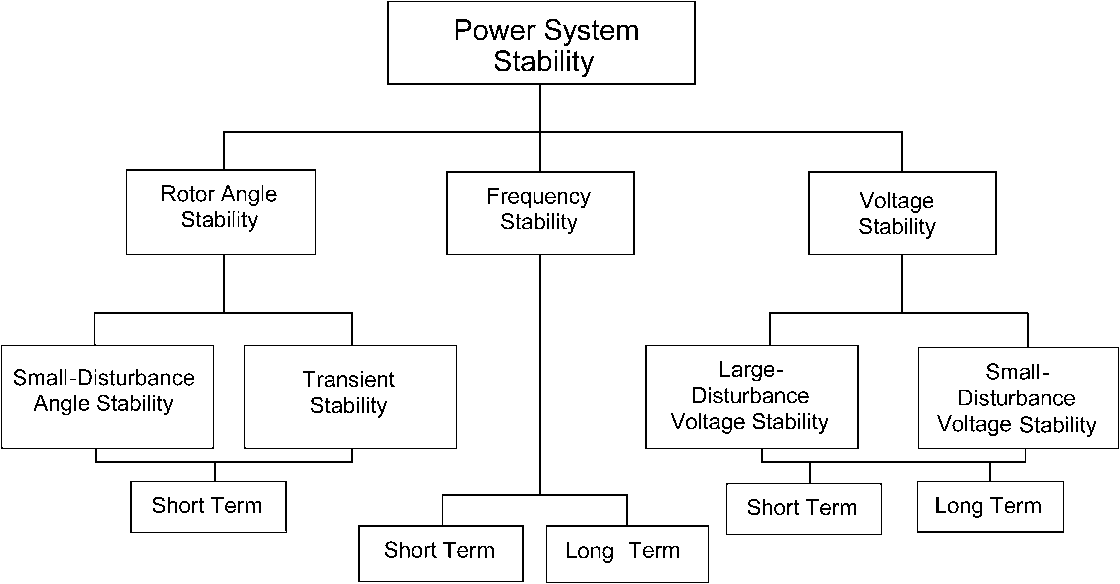
\includegraphics[width=0.9\textwidth]{figurer/Classification_of_power_system_stability}
	\caption{Klassificering af systemstabilitet}
	\label{fig:Overview}
\end{figure}

I dette projekt er det hovedsageligt relevant at undersøge implementeringen af batteriers effekt på nettets frekvensstabilitet og spændingsstabilitet. Dette skyldes at frekvensstabilitet hænger sammen med forholdet mellem produktion og belastning af nettet og spændingsstabilitet hænger sammen med belastningen af nettet, samt kompensering af reaktiv effekt. Rotorvinkelstabilitet er primært relateret til synkron generatorers evne til at forblive synkroniseret med nettet under fejl og vil derfor ikke være et fokus i dette projekt. \\
En forklaring af de stabilitetsproblemer der kan forekomme i forbindelse med frekvensstabilitet og spændingsstabilitet er derfor gennemgået i de følgende afsnit.

\chapter{Frekvensstabilitet}
% !TEX root = ../SYSprojektrapport.tex
% SKAL STÅ I TOPPEN AF ALLE FILER FOR AT MASTER-filen KOMPILERES 

\label{Frekvensstabilitet}

Frekvensstabilitet dækker over et elektrisk systems evne til at opretholde eller hurtigt genoprette systemfrekvensen, selvom systemet påvirkes af forstyrrelse, der vil resulterer i ubalance mellem produktion og belastning. Systemet skal altså kunne reguleres således at der igen opnåes balance mellem produktion og belastning i systemet, uden signifikant tab af belastning.\\
Vedvarende frekvensustabilitet vil føre til udkobling af produktionsenheder og forbrugere.

Frekvensstabilitet inddeles i \textit{short term} og \textit{long term} stabilitetsproblemer, som vist på figur \ref{fig:Overview}.\\
\textit{Short term} har en varighed på op til 1 minut og defineres som pludselige ændringer i belastningsforholdet. Dette kunne være tab af en større generationsenhed, en transmissionslinje eller en stor forbruger. \textit{Short term} problemer kan udvikle sig til \textit{long term}, hvis systemet, med de umiddelbare tilgængelige reguleringsreserver, ikke formår at skabe balance mellem produktion og belastning igen.\\
\textit{Long term} har en varighed fra 1 minut til flere timer og defineres som længerevarende afvigelser fra den nominelle systemfrekvens. Et \textit{long term} problem kunne opstå gennem mistiming af reguleringen på et stort synkron kraftværk grundet en forudset ændring i produktionen fra vedvarende energikilder i systemet, som følge af vejrændringer.
Typiske reguleringshastigheder er for et kulkraftværk 1\% i minuttet og for et gaskraftværk 10-15\% i minuttet.

\subsection{Frekvensregulering og kontrol}
Frekvensstabiliteten opretholdes i normal drift af elnettet gennem handel af elektricitet. Dette sker på timebasis og elektricitetsmarkedet er derfor ansvarlig for at produktionen matcher det forbrug markedet forventer. Ved ubalance i belastningsforholdet har Transmission System Operatoren (TSO) - i Danmark er det Energinet.dk - ansvaret for regulering af produktionen. I ENTSO-E Policy 1 defineres fire forskellige kontroltyper til at opretholde den nominelle systemfrekvens.

\begin{description}
	\item[Primær kontrol] Det enkelte kraftværks egen regulering. Kan aktiveres på sekunder.
	\item[Sekundær kontrol] Midlertidige produktionsreserve, styret af TSO'en, der kan aktiveres på sekunder/minutter med en varighed på ca 15 minutter.
	\item[Tertiær kontrol] Manuelt aktiverede produktionsreserve, styret af TSO'en. Anvendt til længerevarende ustabilitet.
	\item[Time kontrol] Handel på energimarkedet overvåges af TSO'en for at forudse behov for regulering af produktionen.
\end{description}

Måden de forskellige kontrolreserver interagerer med hinanden på kan illustres som vist på figur \ref{fig:Frekvenskontrol}\footnote{ENTSO-E Policy 1}. En afvigelse fra systemfrekvensen vil føre til aktivering af den primære kontrol, for at undgå tab af synkrone generationsenheder og stabilisere frekvensen ved et nyt arbejdspunkt indenfor grænseværdierne for nominel systemfrekvens. Derefter vil den sekundære kontrol aktiveres for at genoprette den nominelle systemfrekvens. Hvis den sekundære kontrol ikke formår at genoprette systemfrekvensen eller hvis generationsenheder er blevet tabt aktiveres den tertiære kontrol. Den tertiære kontrol dækker også over planlagte aktivering/regulering af produktionsenheder, der vil blive anvendt ved tab af større generationsenheder i forbindelse med forstyrrelsen/fejlen.

\begin{figure}[H] % (alternativt [H])
	\centering
	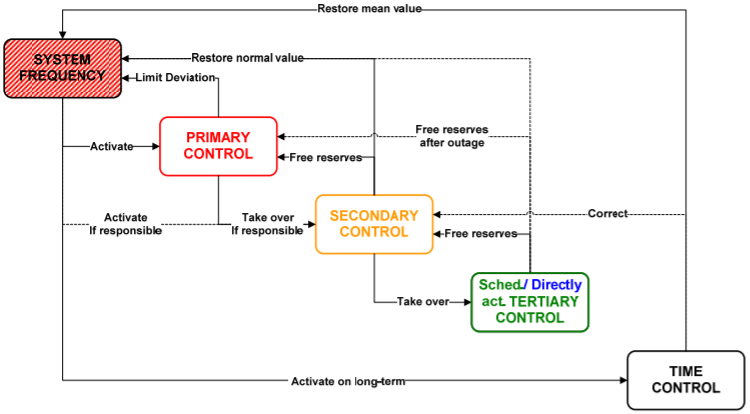
\includegraphics[width=0.9\textwidth]{figurer/Frekvenskontrol}
	\caption{Skematisk overblik over aktiveringen af kontrolreserver til frekvensregulering}
	\label{fig:Frekvenskontrol}
\end{figure}

ENTSO-E Policy 1 nedsætter også nogle krav til reservekapaciteten i det centraleuropæiske elnet. Vigtige krav er at den primære kontrol skal aktiveres ved frekvensafvigelser på $\pm$20mHz og den skal være fuldt ud aktiveret ved afvigelser på $\pm$200mHz. Størrelsen af den primære reserve bliver fastsat årligt og er på 3000MW. Den primære reserve er normeret fordelt på kraftværker i hele det centraleuropæiske elnet.

Den sekundære kontrol implementeres som en Load Frequency Control (LFC) struktur, som vist på figur \ref{fig:sekundaerkontrol}.

\begin{figure}[H]
	\centering
	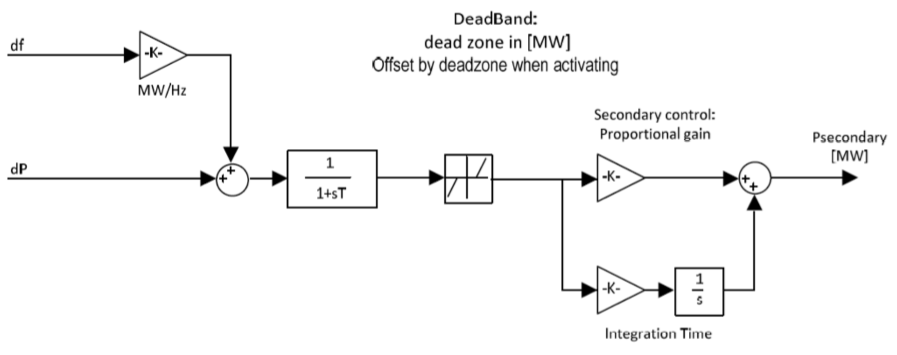
\includegraphics[width=0.9\textwidth]{figurer/Sekundaer_kontrol}
	\caption{LFC struktur}
	\label{fig:sekundaerkontrol}
\end{figure}

Ændringen i frekvens sammenholdes med ændringen i aktiv effekt gennem en K-faktor, der beregnes ud fra et område i systemets afvigelse fra systemfrekvensen efter effektreguleringen pga. aktivering af den primære kontrol. Den samlede påkrævede effektregulering filtreres herefter og hvis afvigelsen i frekvens er udenfor et dødbåndsområde vil en PI regulator regulerer den generede effekt, sådan at systemfrekvensen kan genoprettes.

Et begreb der er relevant for et systems robusthed overfor forstyrrelser, der vil påvirke frekvensen, er inerti. Dette skyldes at inerti har betydning for hvor hurtigt et system reagerer overfor ændringer. Et system med stor inerti vil have en længere responstid på forstyrrelse og frekvensændringen vil derfor ske langsommere. Dette er fordelagtigt, da det stiller mindre krav til hvor hurtigt den primære respons skal reagere. Typisk kommer inerti i elnettet fra synkrone maskiner. Nyere vedvarende energikilder er typisk koblet til nettet gennem en frekvensomformer og bidrager derfor ikke med naturlig inerti. Der forskes derfor i hvordan kontrollen af frekvensomformere kan designes til at kunne generere "kunstig inerti". I dag anvendes der også synkron kondensere til at tilføre elnettet inerti.


\subsection{Batterier som aktivt netelement}

Måden hvorpå batterier i elnettet kan bidrage til at stabilisere systemfrekvensen er at de både kan absorbere og genere effekt afhængigt af behovet og deres opladningstilstand. Dette kan give fordele i et elnet, hvor andelen er vedvarende energikilder er stor og derved har mindre reguleringsreserve i situationer med utilstrækkeligt vejr.

Her kan batterier fungere som både primær og sekundær reserve grundet den hurtige reguleringsmulighed der er i et rent elektrisk system. Et husstandsbatterier har en typisk kapacitet på 14kWh og kan levere 5kW nominelt og 7kW peak\footnote{https://www.tesla.com/da\_DK/powerwall}. Derfor vil enkelte husstandsbatterier ikke kunne bidrage særlig meget til balancering af produktion og forbrug, men en samling af mange husstandsbattier, en såkaldt aggrering, vil kunne bidrage med betydelig effekt. Dette kombineret med muligheden for at oplade batterierne i perioder med stor produktion fra grønne generationsenheder, så deres kapacitet er til rådighed i perioder med lav produktion fra grønne produktionsenheder kan tilføre den nødvendige fleksibilitet til elnettet for at kunne opretholde systemfrekvensen i et elnet med stor andel af vedvarende energikilder.

Placeringen og typen af batterierne forventes for frekvensstabiliteten at være ubetydelig, da den den generede effekt bare skal matche den absorberede for systemet for at opretholde den nominelle systemfrekvens. Det forventes heller ikke at have betydning for inertien i systemet hvor batterierne implementeres, da batterier er ikke roterende enheder og derfor ikke vil bidrage med naturlig inerti. En batteri inverter kunne muligvis designes til at kunne genere "kunstig inerti", men dette vil ikke blive undersøgt i dette projekt.




\chapter{Spændingsstabilitet}
% !TEX root = ../prj4projektrapport.tex
% SKAL STÅ I TOPPEN AF ALLE FILER FOR AT MASTER-filen KOMPILERES 

\chapter{Kortslutningseffekt}
% !TEX root = ../prj4projektrapport.tex
% SKAL STÅ I TOPPEN AF ALLE FILER FOR AT MASTER-filen KOMPILERES 

\chapter{Model og validering}
% !TEX root = ../SYSprojektrapport.tex
% SKAL STÅ I TOPPEN AF ALLE FILER FOR AT MASTER-filen KOMPILERES 


\label{Modelopbygning}
I dette kapitel beskrives modellen og det underbyggende data, der anvendes til simuleringen af de omtalte cases. Modellen valideres igennem spændingsfalds- og kortslutningsberegninger.

\section{Model}

For at undersøge husstandsbatterier indflydelse i et elnet er der simuleret 5 byer med ca. 2000 hustande, der alle har et batteri installeret. Hver husstand er sat til at have et gennemsnitligt dagligt forbrug på 14kWh\footnote{https://orsted.dk/Privat/Faa-en-lavere-regning/Kom-godt-i-gang-og-spar-paa-energien/Test-dit-gennemsnitsforbrug/Elforbrug}. Det giver et gennemsnitlig forbrug på 1183kW per by. For at finde en realistisk maksimal belastning er der taget udgangspunkt i Energinets belastnings- og produktionsinformation for Danmark\footnote{https://www.energidataservice.dk/da\_DK/}. Det er undersøgt hvor stor en del den gennemsnitlige belastning i modellen udgør af Danmarks gennemsnitlige belastning og derved fundet en skaleringsfaktor på 716. Denne skaleringsfaktor er brugt til at finde den samlede maksimale belastning for byerne ved dividere Danmarks maksimale belastning med faktoren. Den maksimale belastning for hver by ligger derved på 1524kW. \\
På figur \ref{fig:Simdis} ses distributionsnettets opbygning der er lavet som en ringforbindelse fra \textit{Distribution busbar}, med en ekstra tværgående linje. Ved hver by er placeret en transformer der transformere spændingen fra 10kV til 0,4kV. Hver by er simplificeret til en belastning, et batteri og et solcelle anlæg. Den maksimale batteri kapacitet er fundet i forhold til at hver hustand har monteret en Tesla powerwall, der kan levere 5kW, så hver by har en batteri kapacitet på 10000kW. Den maksimale solcelle produktionsmængde er fundet ud fra Energinets oplysninger for hele landet og derefter divideret med skaleringsfaktoren, som giver en maksimal produktion på 912kW per by. 
Kondensatorbanke er tilføjet for at lave reaktiv kompensering i systemet. Disse er dimensioneret så spændingen i byerne under stabile forhold er 1pu.

 
 \begin{figure}[H] % (alternativt [H])
 	\centering
 	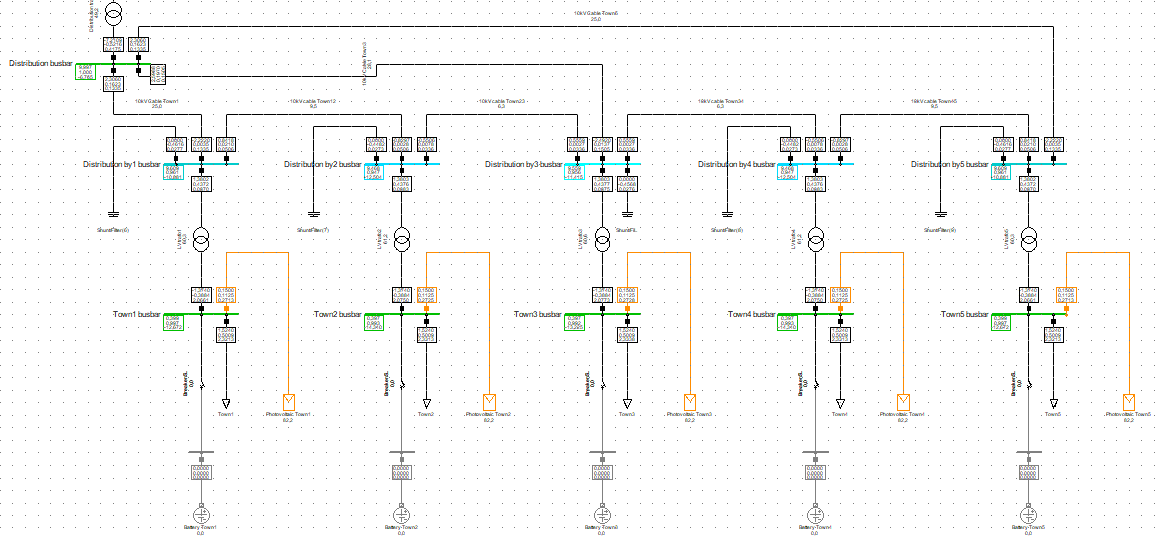
\includegraphics[width=1\textwidth]{figurer/Sim_model_2}
 	\caption{Systemets belastning og distribution}
 	\label{fig:Simdis}
 \end{figure}
    

På figur \ref{fig:SimTrans} ses transmissionsnettet. For at simplificere modellen er al vind- og fossil energi samlet i to generatorer. Størrelsen af vind generatoren er valgt ud fra den gennemsnitlige produktion af vindenergi i Danmark. Vindmølle generatoren producerer derved 2MW. Den fossile generator er sat som referencemaskine og ændre sin produktion i forhold til belastningen i nettet. Energien transformeres først op til et 150kV transmissions net og derefter til 60kV. 60kV transmissionen er lavet med 2 redundante kabler så det kan undersøges hvad der sker, hvis det ene kable falder ud. Til sidst transformeres spændingen ned til distributions niveauet. Ydermere er der placeret en stor batterienhed på 60kV busbaren for at kunne undersøge forskellen mellem husstandsbatterier og en centralt placeret batteripark.

Generatorer, kabler og transformere er lavet som simplificeret modeller med generelle værdier for de enkelte komponenter samt tilpasset for spænding og belastning i de forskellige niveauer. Der er fundet information i bøgerne \textit{Power System Control and Stability} og \textit{Elektrische Energieversorgun}.

 

\begin{figure}[H] % (alternativt [H])
	\centering
	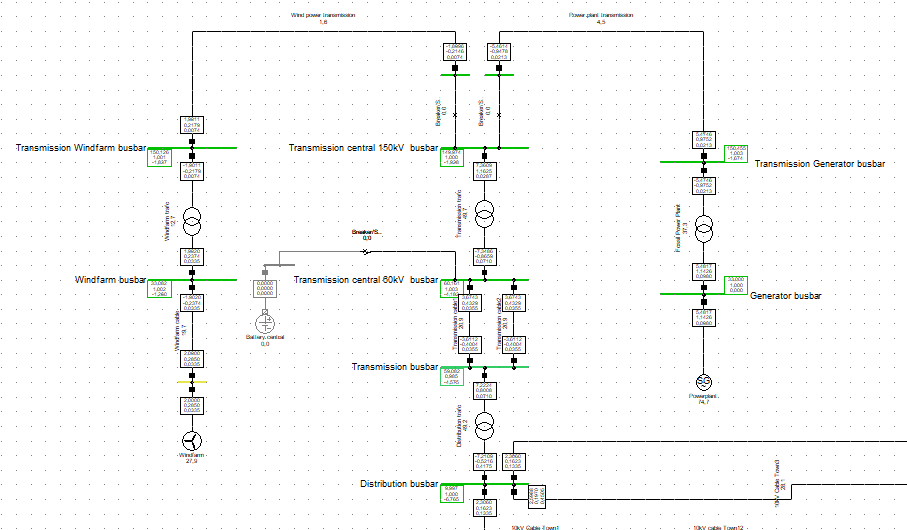
\includegraphics[width=1\textwidth]{figurer/Sim_model_1}
	\caption{systemets produktion transmission}
	\label{fig:SimTrans}
\end{figure}

% !TEX root = ../SYSprojektrapport.tex
% SKAL STÅ I TOPPEN AF ALLE FILER FOR AT MASTER-filen KOMPILERES 

\label{Validering}

\chapter{Simulering}
% !TEX root = ../SYSprojektrapport.tex
% SKAL STÅ I TOPPEN AF ALLE FILER FOR AT MASTER-filen KOMPILERES 

\label{Simulering}

\section{Case 1: Husstandsbatteriers evne til at stabilisere elnettet ved fejl på nettet}
For at simulere case 1 er anvendt et scenarie, hvor systemet er fuldt belastet, dvs. hver by trækker 1,524MW med pf 0,95 lagging. Efter 10s mister systemet kablet 10kV Cable Town5 ved en udkobling. Dette betegnes som en small disturbance fejl der vil skabe short term ubalance i powerflowet.\\
Vindmølleparken generer 2MW med pf 0,99 lagging, solcellerne i hver by levere 0,15MW med pf 0.8 lagging og synkron generatoren er reference maskine.\\
Case 1 simuleres i fire forskellige tilstande.

\begin{description}
	\item[Tilstand 1] Alle batterierne er frakoblet.
	\item[Tilstand 2] Batteriet i Town4 leverer 0,25MW og batteriet i Town5 leverer 0,5MW. Begge med pf 0,95 lagging.
	\item[Tilstand 3] Batteriet i Town4 leverer 0,5MW og batteriet i Town5 leverer 1MW. Begge med pf 0,95 lagging.
	\item[Tilstand 4] Batteriet i Town4 leverer 0,75MW og batteriet i Town5 leverer 1,5MW. Begge med pf 0,95 lagging.
\end{description}

Parametrene der overvåges er for synkron generatoren P, Q og V.
For batterierne i Town4 og Town5 P og Q. Samt V for Transmission 60kV busbar, Town1 busbar, Town2 busbar, Town3 busbar, Town4 busbar og Town5 busbar.
Derudover overvåges systemfrekvensen.

\section{Case 2: Husstandsbatteriers evne til at absorbere overproduktion}
For at simulere case 2 er anvendt et scenarie, hvor systemet er fuldt belastet, dvs. hver by trækker 1,524MW med pf 0,95 lagging. Efter 10s mister systemet Town2 ved en udkobling ved Distribution by2 busbar. Dette betegnes som en large disturbance fejl, der vil normalt vil skabe en long term ubalance i powerflowet. I case 2 simuleres kun den short term påvirkning det vil have på systemet, da det stadig vil give et indblik i batteriernes evne til at absorbere overproduktion.\\
Vindmølleparken generer 2MW med pf 0,95 lagging, solcellerne i hver by levere 0,15MW med pf 0.8 lagging og synkron generatoren er reference maskine.\\
Case 2 simuleres i to forskellige tilstande.

\begin{description}
	\item[Tilstand 1] Alle batterierne er frakoblet.
	\item[Tilstand 2] Batterierne i alle byer kobles ind 0,5s efter fejlen og absorberer 0,304MW som kompensation for tabet af byen. Alle med pf 0,95 lagging.
\end{description}

Parametrene der overvåges er for synkron generatoren P, Q og V.
For batterierne i alle 5 byer P og Q. Samt V for Transmission 60kV busbar, Town1 busbar, Town2 busbar, Town3 busbar, Town4 busbar og Town5 busbar.
Derudover overvåges systemfrekvensen.

\section{Case 3: Husstandsbatteriers evne til at udglatte produktion over døgnet}
For at simulere case 3 er anvendt et scenarie, hvor systemet er fuldt belastet, dvs. hver by trækker 1,524MW med pf 0,95 lagging, samt at kablet Transmission cable2 er koblet ud pga. vedligeholdelse. Efter 10s mister systemet vindmølleparken ved en udkobling ved Transmission central 160kV busbar. Dette betegnes som en large disturbance fejl, der vil normalt vil skabe en long term ubalance i powerflowet eller muligvis blackout i større dele at systemet. I case 3 simuleres kun den short term påvirkning det vil have på systemet, da det stadig vil give et indblik i batteriernes evne til at kompensere for mistet produktion.\\
Vindmølleparken generer 2MW med pf 0,95 lagging, solcellerne i hver by levere 0,15MW med pf 0.8 lagging og synkron generatoren er reference maskine.\\
Case 3 simuleres i fire forskellige tilstande.

\begin{description}
	\item[Tilstand 1] Alle batterierne er frakoblet.
	\item[Tilstand 2] Alle batterier leverer 0,5MW med pf 0,95 lagging.
	\item[Tilstand 3] Alle batterier leverer 1MW med pf 0,95 lagging.
	\item[Tilstand 4] Alle batterier leverer 1,35MW (Byerne kan betegnes som selvforsynende) med pf 0,95 lagging.
\end{description}

Parametrene der overvåges er for synkron generatoren P, Q og V.
For batterierne i alle 5 byer P og Q. Samt V for Transmission 60kV busbar, Town1 busbar, Town2 busbar, Town3 busbar, Town4 busbar og Town5 busbar.
Derudover overvåges systemfrekvensen.

\section{Case 4: Husstandsbatteriers stabiliserende effekt af elnettet kontra en central batteripark}
Case 4 er den samme som case 3, bortset fra at batteriparken anvendes i stedet for husstandsbatterierne.
Case 4 simuleres i fire forskellige tilstande.

\begin{description}
	\item[Tilstand 1] Batteripark er frakoblet.
	\item[Tilstand 2] Batteriparken leverer 2,5MW med pf 0,95 lagging.
	\item[Tilstand 3] Batteriparken leverer 5MW med pf 0,95 lagging.
	\item[Tilstand 4] Batteriparken leverer 6,75MW med pf 0,95 lagging.
\end{description}

Parametrene der overvåges er for synkron generatoren P, Q og V.
For batteriparken P og Q. Samt V for Transmission 60kV busbar, Town1 busbar, Town2 busbar, Town3 busbar, Town4 busbar og Town5 busbar.
Derudover overvåges systemfrekvensen.


\chapter{Resultat og diskussion}
% !TEX root = ../SYSprojektrapport.tex
% SKAL STÅ I TOPPEN AF ALLE FILER FOR AT MASTER-filen KOMPILERES 

\label{ResultatOgDiskussion}

\section{Case 1: Husstandsbatteriers evne til at stabilisere elnettet ved fejl på nettet}
I dette afsnit præsenteres resultater for simuleringen af case 1 iht. beskrivelsen i afsnit \ref{SimCase1}. I alle fire tilstande er spændingsændringen ved Town5 busbar (rød linje) og Transmission central 60kV busbar (Grøn linje) samt frekvensændringen på Transmission central 60kV busbar (Grøn linje), præsenteret på hhv. spændingsgraf og frekvensgraf. Derudover er der lavet opsamling over spænding samt effektoverførelse andre relevante steder i systemet i tabel \ref{fig:C1Overview}. \\ \\

\textbf{Tilstand 1: Alle batterierne er frakoblet.}
\begin{figure}[H]
	\centering
	\begin{minipage}[b]{0.48\textwidth}
		\centering
		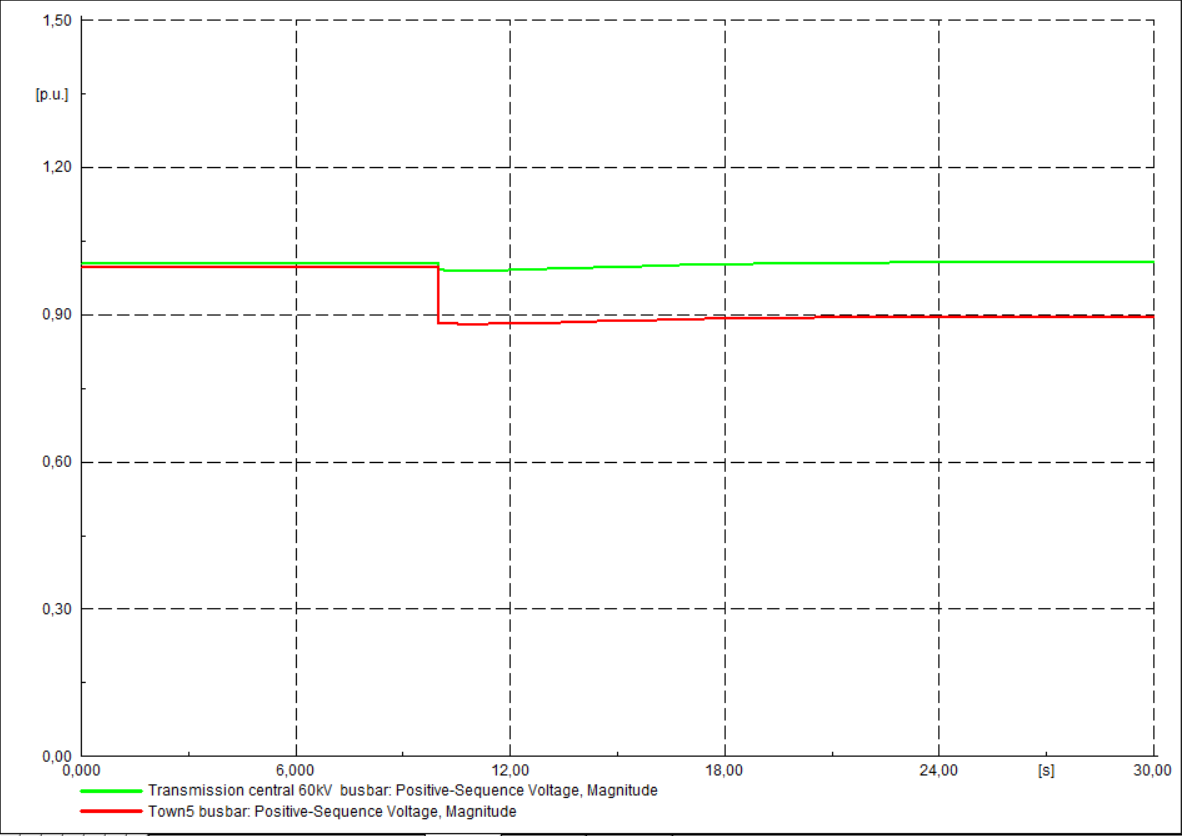
\includegraphics[width=1.00\textwidth]{figurer/SmallDisturbance/Voltage1} % Venstre billede
	\end{minipage}
	\hfill
	\begin{minipage}[b]{0.48\textwidth}
		\centering
		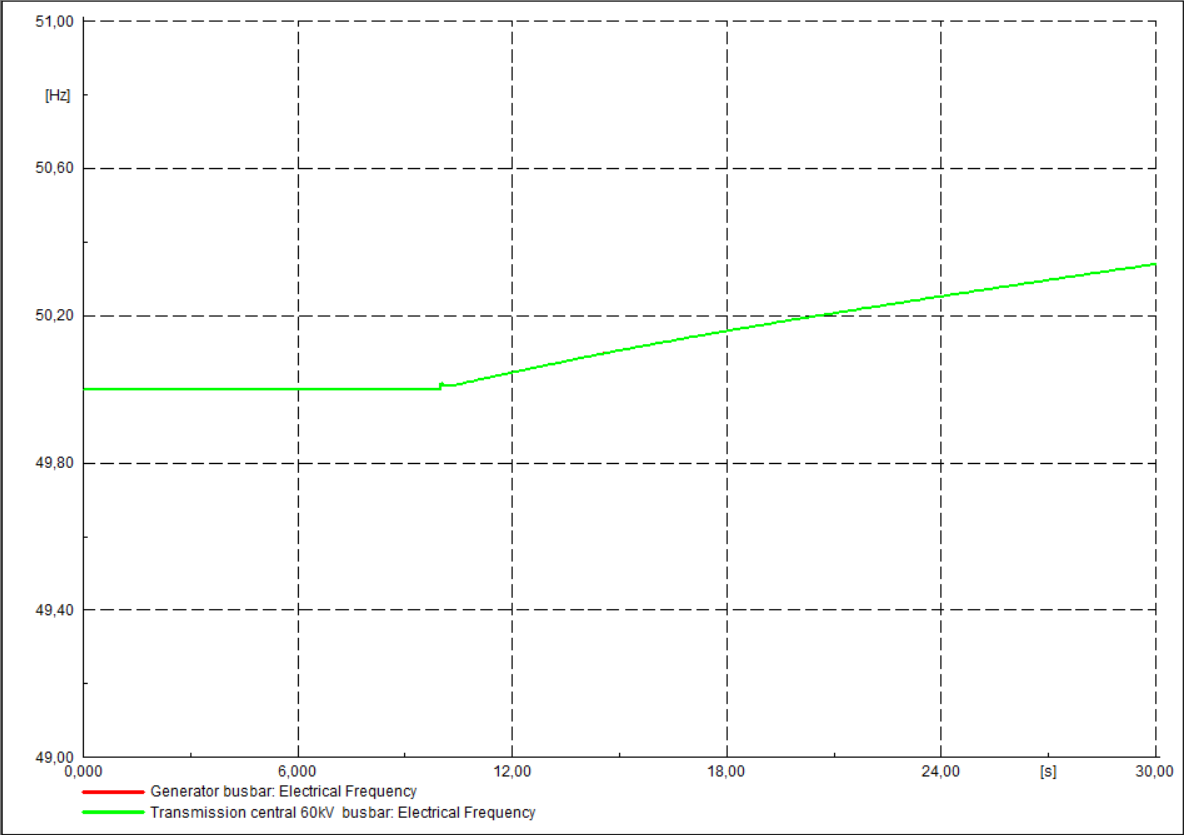
\includegraphics[width=1.00\textwidth]{figurer/SmallDisturbance/Freq1} % Højre billede
	\end{minipage}
	\\ % Figurtekster og labels
	\begin{minipage}[t]{0.48\textwidth}
		\caption{Case 1, Tilstand 1, Spændingsgraf} % Venstre figurtekst og label
		\label{fig:C1T1V}
	\end{minipage}
	\hfill
	\begin{minipage}[t]{0.48\textwidth}
		\caption{Case 1, Tilstand 1, Frekvensgraf} % Højre figurtekst og label
		\label{fig:C1T1F}
	\end{minipage}
\end{figure}

\textbf{Tilstand 2: Batteriet i Town4 leverer 0,25MW og batteriet i Town5 leverer 0,5MW. Begge med pf 0,95 lagging.}
\begin{figure}[H]
	\centering
	\begin{minipage}[b]{0.48\textwidth}
		\centering
		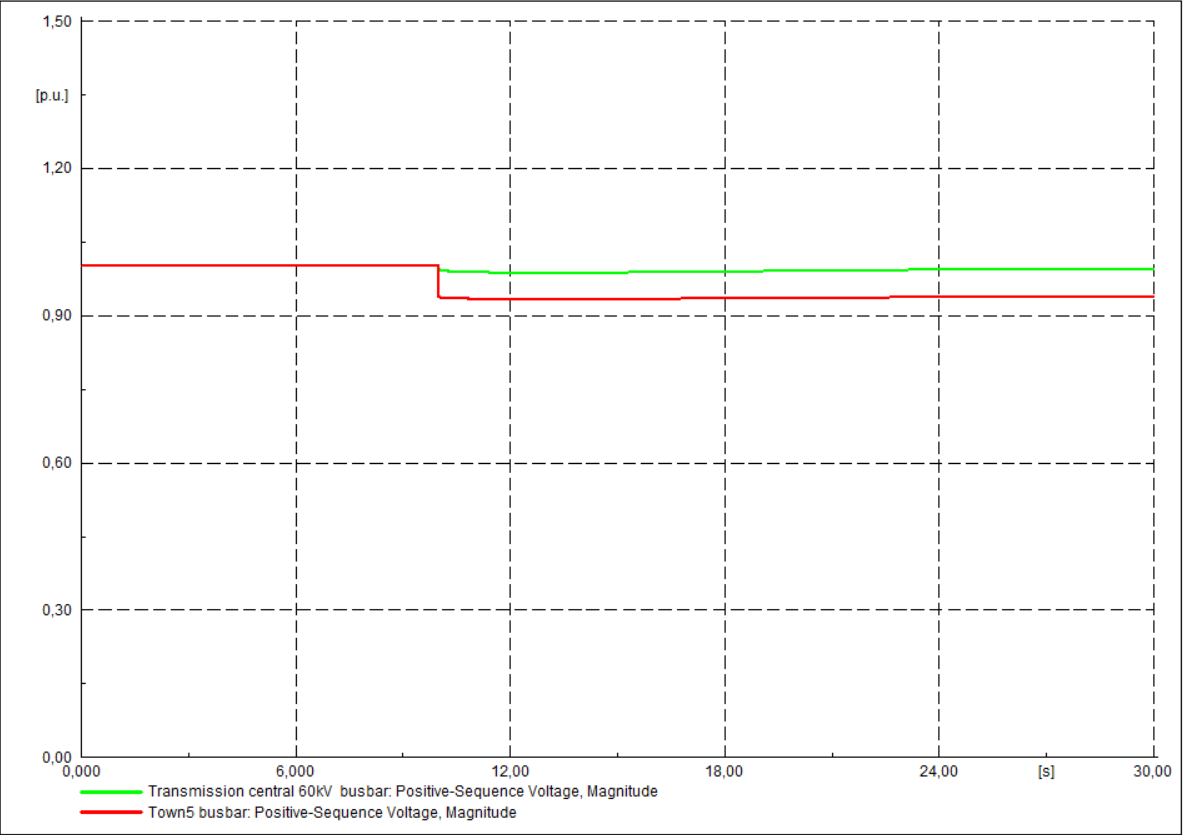
\includegraphics[width=1.00\textwidth]{figurer/SmallDisturbance/Voltage2} % Venstre billede
	\end{minipage}
	\hfill
	\begin{minipage}[b]{0.48\textwidth}
		\centering
		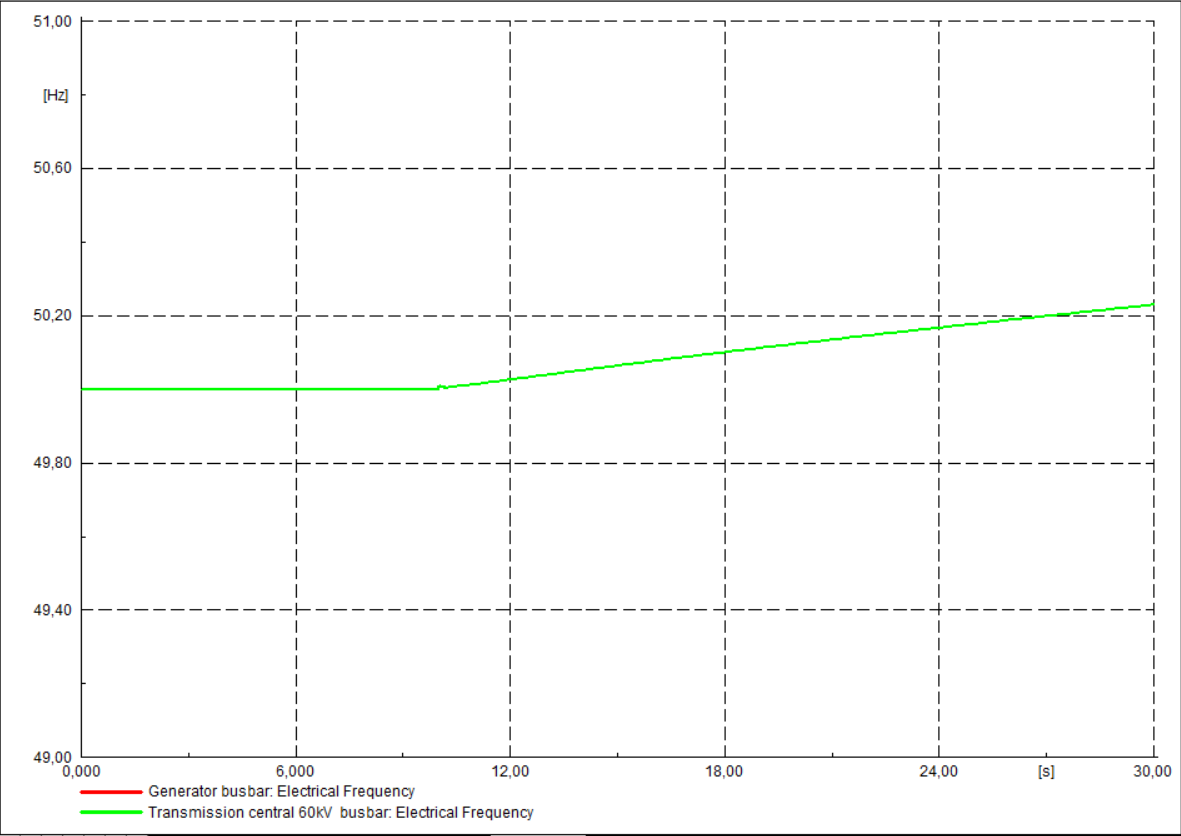
\includegraphics[width=1.00\textwidth]{figurer/SmallDisturbance/Freq2} % Højre billede
	\end{minipage}
	\\ % Figurtekster og labels
	\begin{minipage}[t]{0.48\textwidth}
		\caption{Case 1, Tilstand 2, Spændingsgraf} % Venstre figurtekst og label
		\label{fig:C1T2V}
	\end{minipage}
	\hfill
	\begin{minipage}[t]{0.48\textwidth}
		\caption{Case 1, Tilstand 2, Frekvensgraf} % Højre figurtekst og label
		\label{fig:C1T2F}
	\end{minipage}
\end{figure}

\textbf{Tilstand 3: Batteriet i Town4 leverer 0,5MW og batteriet i Town5 leverer 1MW. Begge med pf 0,95 lagging.}
\begin{figure}[H]
	\centering
	\begin{minipage}[b]{0.48\textwidth}
		\centering
		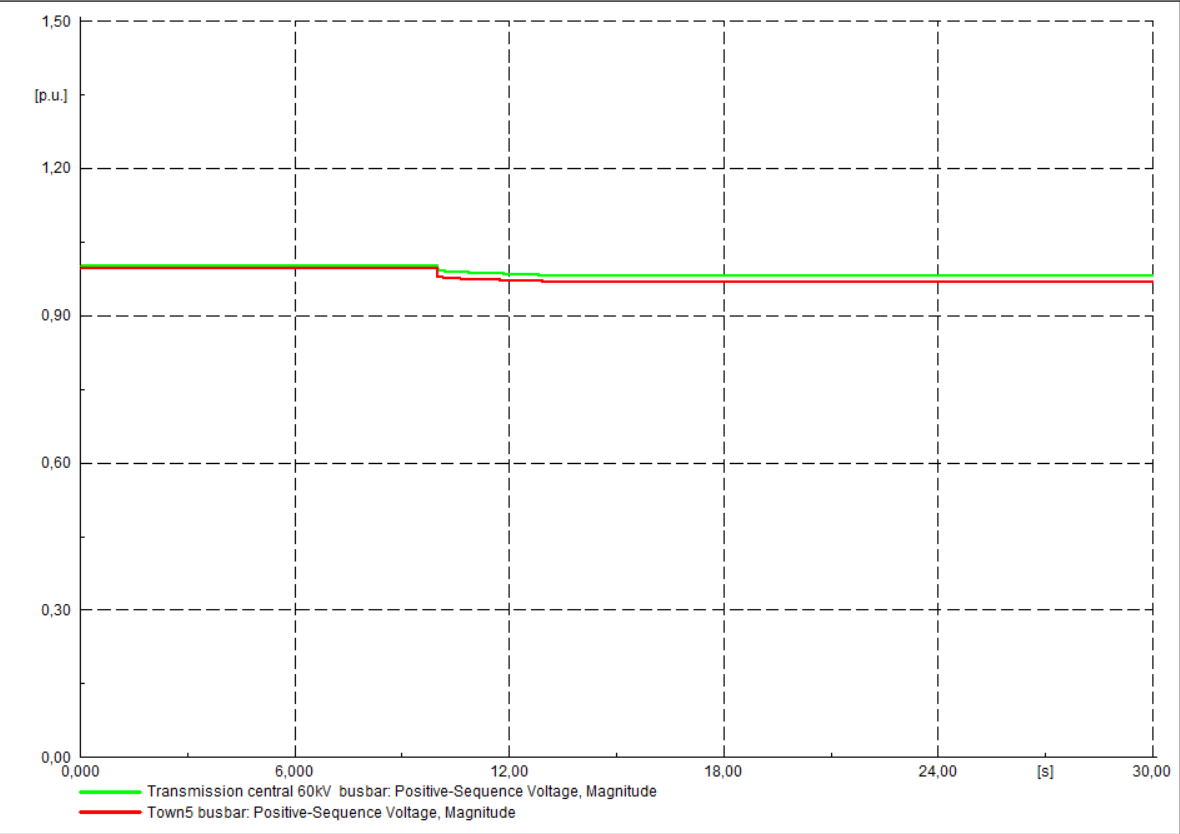
\includegraphics[width=1.00\textwidth]{figurer/SmallDisturbance/Voltage3} % Venstre billede
	\end{minipage}
	\hfill
	\begin{minipage}[b]{0.48\textwidth}
		\centering
		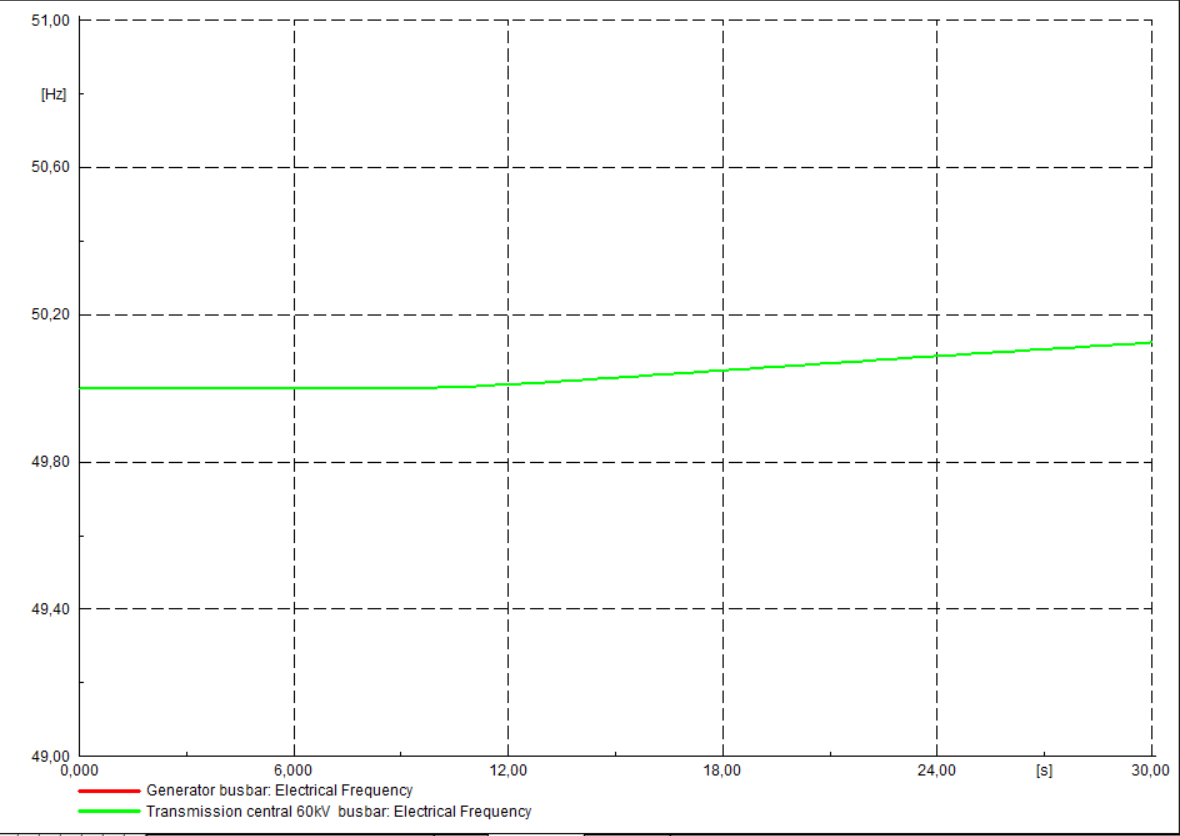
\includegraphics[width=1.00\textwidth]{figurer/SmallDisturbance/Freq3} % Højre billede
	\end{minipage}
	\\ % Figurtekster og labels
	\begin{minipage}[t]{0.48\textwidth}
		\caption{Case 1, Tilstand 3, Spændingsgraf} % Venstre figurtekst og label
		\label{fig:C1T3V}
	\end{minipage}
	\hfill
	\begin{minipage}[t]{0.48\textwidth}
		\caption{Case 1, Tilstand 3, Frekvensgraf} % Højre figurtekst og label
		\label{fig:C1T3F}
	\end{minipage}
\end{figure}

\textbf{Tilstand 4: Batteriet i Town4 leverer 0,75MW og batteriet i Town5 leverer 1,5MW. Begge med pf 0,95 lagging.}
\begin{figure}[H]
	\centering
	\begin{minipage}[b]{0.48\textwidth}
		\centering
		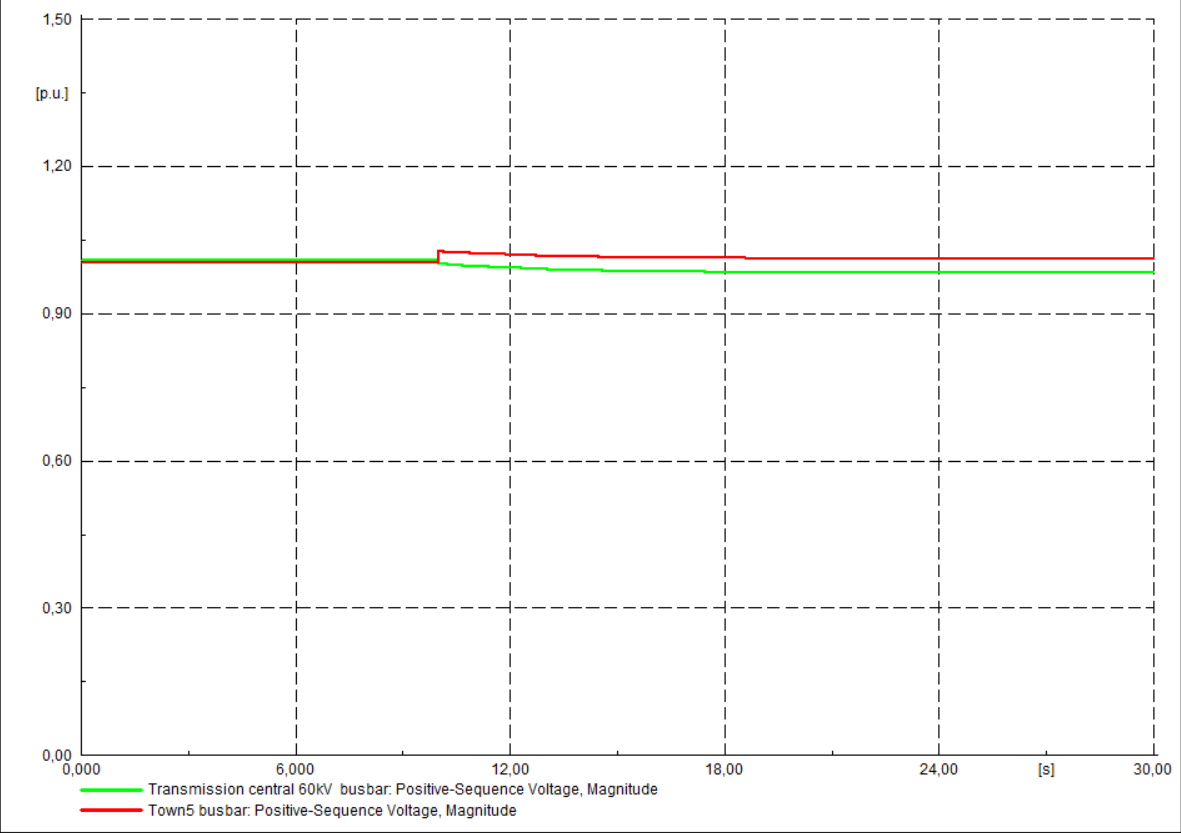
\includegraphics[width=1.00\textwidth]{figurer/SmallDisturbance/Voltage4} % Venstre billede
	\end{minipage}
	\hfill
	\begin{minipage}[b]{0.48\textwidth}
		\centering
		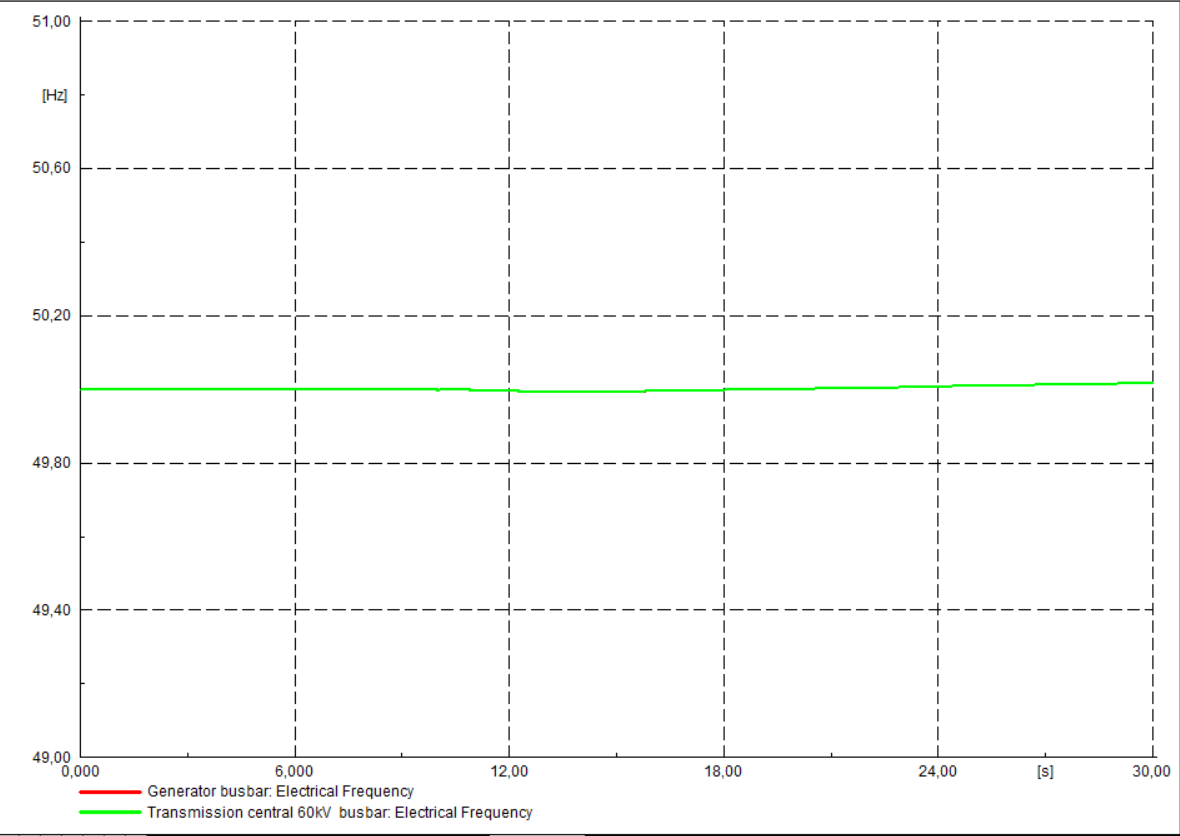
\includegraphics[width=1.00\textwidth]{figurer/SmallDisturbance/Freq4} % Højre billede
	\end{minipage}
	\\ % Figurtekster og labels
	\begin{minipage}[t]{0.48\textwidth}
		\caption{Case 1, Tilstand 4, Spændingsgraf} % Venstre figurtekst og label
		\label{fig:C1T4V}
	\end{minipage}
	\hfill
	\begin{minipage}[t]{0.48\textwidth}
		\caption{Case 1, Tilstand 4, Frekvensgraf} % Højre figurtekst og label
		\label{fig:C1T4F}
	\end{minipage}
\end{figure}

\textbf{Tilstandsoverblik}
\begin{figure}[H] % (alternativt [H])
	\centering
	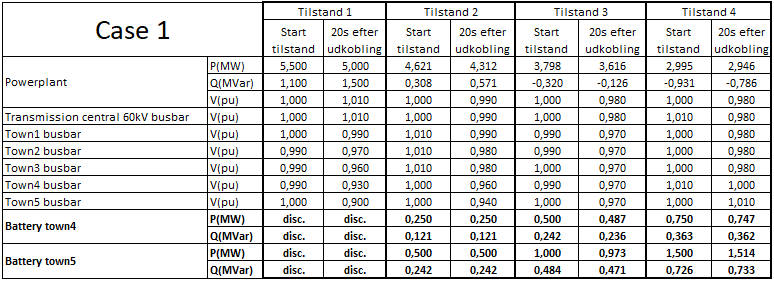
\includegraphics[width=1\textwidth]{figurer/SmallDisturbance/Overview}
	\caption{Overblik for spænding og effektoverførelse i nettet}
	\label{fig:C1Overview}
\end{figure}


I de 3 første tilstande observeres et spændingsfald ved Town5 busbar, når linjen 10kV Cable Town5 udkobles. Størrelsen afhænger af batteriernes effektbidrag. I tilstand 4 ses det at spændingen ved Town5 busbar stiger ved udkoblingen. Spænding ved Transmissions central 60kV busbar forbliver konstant på ca. 1pu i alle tilstande. Spændingsfaldet i tilstandende 1 - 3 er forventet, fordi tabet af den redundante linje vil øge kilde impedansen set fra Town5 busbar. Spændingsfaldet bliver mindre desto mere batteri effektbidrag pga. den reduceret strøm i transmissions og distributions kabler. Spændingsstigningen i tilstand 4 kan forklares ved at Town5 har større produktion end forbrug, derved vil den levere effekt til resten af systemet. Ved tab af 10kV Cable Town5, bliver load impedansen set fra Town5 busbar større og der vil opleves en spændingsstigning ved byens POC.

I de 4 tilstande ses det at frekvensen bliver mere stabilt ved større batteri bidrag. Stigningen på frekvensen i de første tilstande sker fordi at den samlede belastning bliver mindre da spændingen falder, produktionen forsøger at nedregulere, men kan ikke regulere hurtigt nok ift. belastningen. Dette sker ikke i tilstand 4 da spændingen ikke falder.   

% !TEX root = ../SYSprojektrapport.tex
% SKAL STÅ I TOPPEN AF ALLE FILER FOR AT MASTER-filen KOMPILERES 

% !TEX root = ../SYSprojektrapport.tex
% SKAL STÅ I TOPPEN AF ALLE FILER FOR AT MASTER-filen KOMPILERES 

\label{ResultatOgDiskussion2}

\section{Case 2: Husstandsbatteriers evne til at absorbere overproduktion}
I dette afsnit præsenteres resultater for simuleringen af case 2 iht. beskrivelsen i afsnit \ref{SimCase2}. I de 2 tilstande er spændingsændringen ved Town5 busbar (rød linje) og Transmission central 60kV busbar (Grøn linje) samt frekvensændringen på Transmission central 60kV busbar (Grøn linje), præsenteret på hhv. spændingsgraf og frekvensgraf. Derudover er der lavet opsamling over spænding samt effektoverførelse andre relevante steder i systemet i tabel \ref{fig:C2Overview}. \\ \\

\textbf{Tilstand 1: Alle batterierne er frakoblet.}
\begin{figure}[H]
	\centering
	\begin{minipage}[b]{0.48\textwidth}
		\centering
		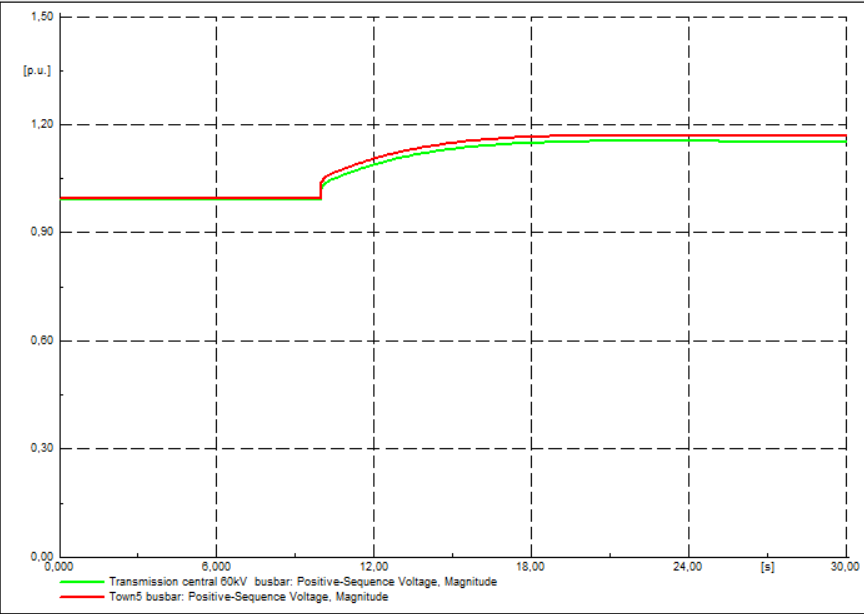
\includegraphics[width=1.00\textwidth]{figurer/LossOfTown/Voltage1} % Venstre billede
	\end{minipage}
	\hfill
	\begin{minipage}[b]{0.48\textwidth}
		\centering
		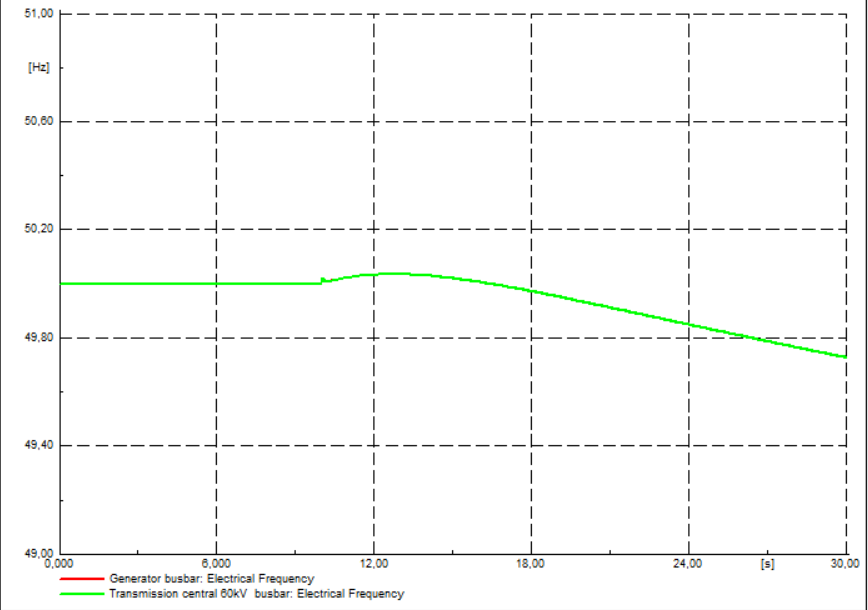
\includegraphics[width=1.00\textwidth]{figurer/LossOfTown/Freq1} % Højre billede
	\end{minipage}
	\\ % Figurtekster og labels
	\begin{minipage}[t]{0.48\textwidth}
		\caption{Case 2, Tilstand 1, Spændingsgraf} % Venstre figurtekst og label
		\label{fig:C2T1V}
	\end{minipage}
	\hfill
	\begin{minipage}[t]{0.48\textwidth}
		\caption{Case 2, Tilstand 1, Frekvensgraf} % Højre figurtekst og label
		\label{fig:C2T1F}
	\end{minipage}
\end{figure}

\textbf{Tilstand 2: Batterierne i alle byer kobles ind 0,5s efter fejlen og absorberer 0,304MW som kompensation for tabet af byen. Alle med pf 0,95}
\begin{figure}[H]
	\centering
	\begin{minipage}[b]{0.48\textwidth}
		\centering
		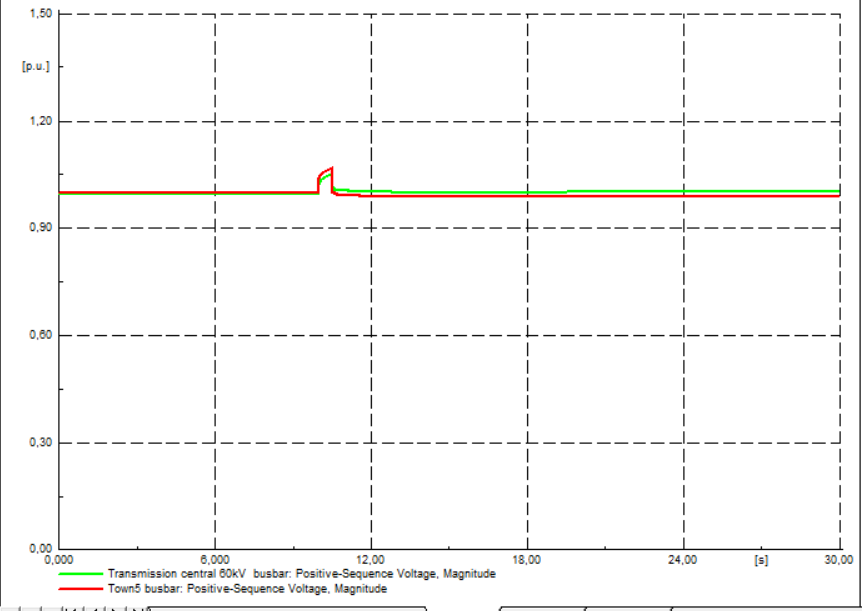
\includegraphics[width=1.00\textwidth]{figurer/LossOfTown/Voltage2} % Venstre billede
	\end{minipage}
	\hfill
	\begin{minipage}[b]{0.48\textwidth}
		\centering
		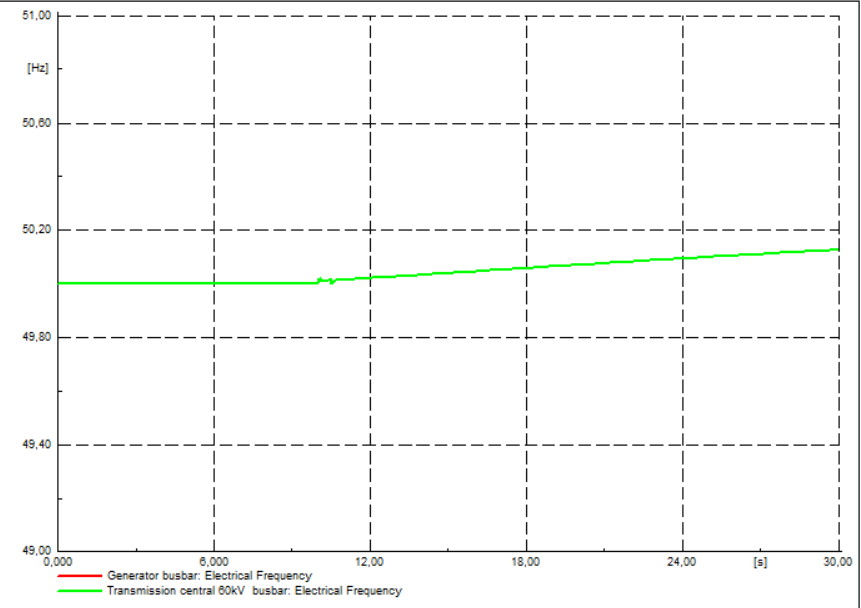
\includegraphics[width=1.00\textwidth]{figurer/LossOfTown/Freq2} % Højre billede
	\end{minipage}
	\\ % Figurtekster og labels
	\begin{minipage}[t]{0.48\textwidth}
		\caption{Case 2, Tilstand 2, Spændingsgraf} % Venstre figurtekst og label
		\label{fig:C2T2V}
	\end{minipage}
	\hfill
	\begin{minipage}[t]{0.48\textwidth}
		\caption{Case 2, Tilstand 2, Frekvensgraf} % Højre figurtekst og label
		\label{fig:C2T2F}
	\end{minipage}
\end{figure}

\textbf{Tilstandsoverblik}
\begin{figure}[H] % (alternativt [H])
	\centering
	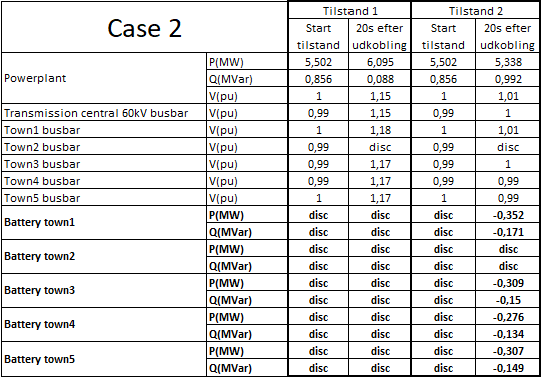
\includegraphics[width=1\textwidth]{figurer/LossOfTown/Overview}
	\caption{Overblik for spænding og effektoverførelse i nettet}
	\label{fig:C2Overview}
\end{figure}

I tilstand 1 ses det at spænding stiger betydeligt ved Town5 busbar og Transmissions central 60kV busbar. I tilstand 2 stiger spændingen kortvarigt indtil batterierne kobles ind. Spænding stiger i tilstand 1 da der er for meget produktion i forhold til belastning. Da batterierne i tilstand 2 påbegynder opladning hurtigt efter tabet af Town2 kompensere de for det manglende belastning og stabilisere derfor spændingen til normal.

Frekvensen starter med at stige lidt pga. den udkoblede belastning. hvorefter den begynder at falde lidt igen. Dette sker formentlig fordi at belastning stiger i de ikke afkoblede byer pga. overspændingen og det ser ikke ud til at Powerfactory tilpasser spændingsniveauet efter at belastningen stiger igen. I tilstand 2 stiger frekvensen formentlig pga. det hurtigt afkoblede produktion og da inertien er ret høj i systemet går der lidt tid inden den tilpasser sig systemet igen.
  

% !TEX root = ../SYSprojektrapport.tex
% SKAL STÅ I TOPPEN AF ALLE FILER FOR AT MASTER-filen KOMPILERES 

\section{Case 3: Husstandsbatteriers evne til at kompensere for tab af produktion}
I dette afsnit præsenteres resultater for simuleringen af case 3 iht. beskrivelsen i afsnit \ref{SimCase1}. I alle fire tilstande er spændingsændringen ved \textit{Town5 busbar} (rød linje) og \textit{Transmission central 60kV busbar} (Grøn linje) samt frekvensændringen på \textit{Transmission central 60kV busbar} (Grøn linje) præsenteret på hhv. spændingsgraf og frekvensgraf. Derudover er der lavet opsamling over spænding samt effektoverførelse andre relevante steder i systemet i tabel \ref{fig:C3Overview}. \\ \\

\newpage
\textbf{Tilstand 1: Alle batterierne er frakoblet.}
\begin{figure}[H]
	\centering
	\begin{minipage}[b]{0.48\textwidth}
		\centering
		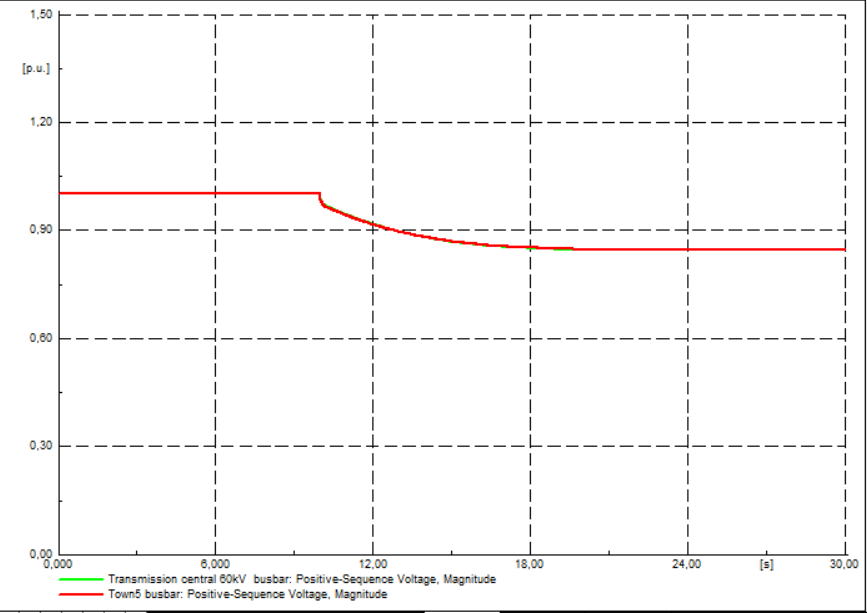
\includegraphics[width=1.00\textwidth]{figurer/LargeDisturbance/Voltage1} % Venstre billede
	\end{minipage}
	\hfill
	\begin{minipage}[b]{0.48\textwidth}
		\centering
		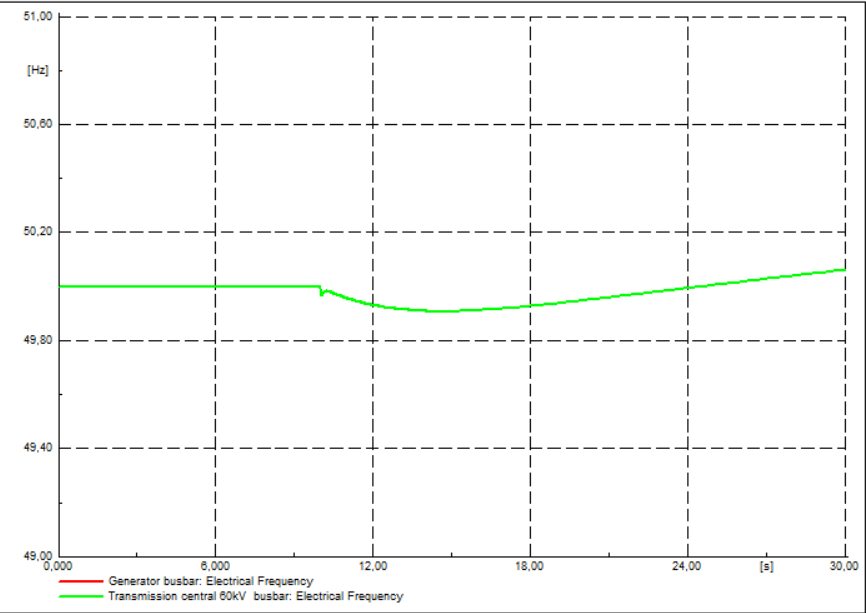
\includegraphics[width=1.00\textwidth]{figurer/LargeDisturbance/Freq1} % Højre billede
	\end{minipage}
	\\ % Figurtekster og labels
	\begin{minipage}[t]{0.48\textwidth}
		\caption{Case 3, Tilstand 1, Spændingsgraf} % Venstre figurtekst og label
		\label{fig:C3T1V}
	\end{minipage}
	\hfill
	\begin{minipage}[t]{0.48\textwidth}
		\caption{Case 3, Tilstand 1, Frekvensgraf} % Højre figurtekst og label
		\label{fig:C3T1F}
	\end{minipage}
\end{figure}

\textbf{Tilstand 2: Alle batterier leverer 0,5MW med pf 0,95 lagging.}
\begin{figure}[H]
	\centering
	\begin{minipage}[b]{0.48\textwidth}
		\centering
		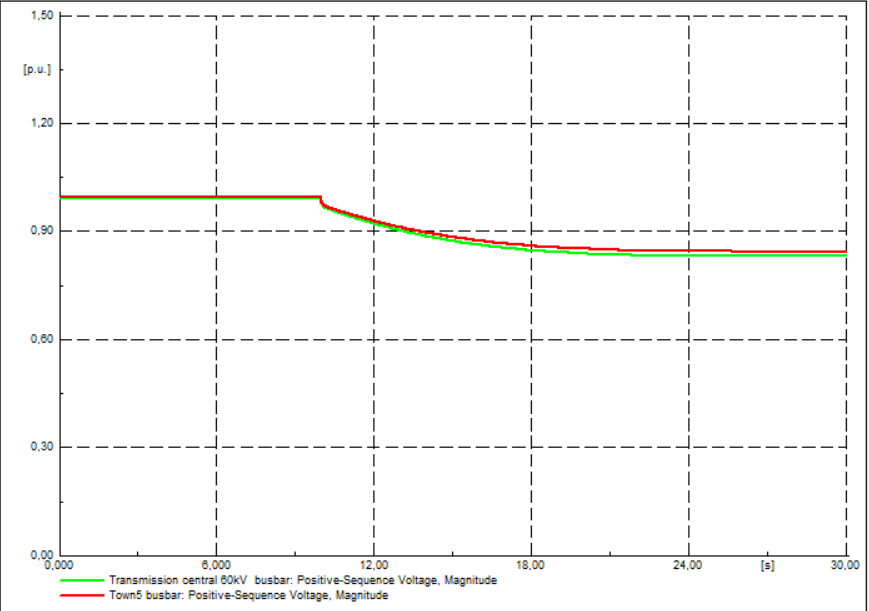
\includegraphics[width=1.00\textwidth]{figurer/LargeDisturbance/Voltage2} % Venstre billede
	\end{minipage}
	\hfill
	\begin{minipage}[b]{0.48\textwidth}
		\centering
		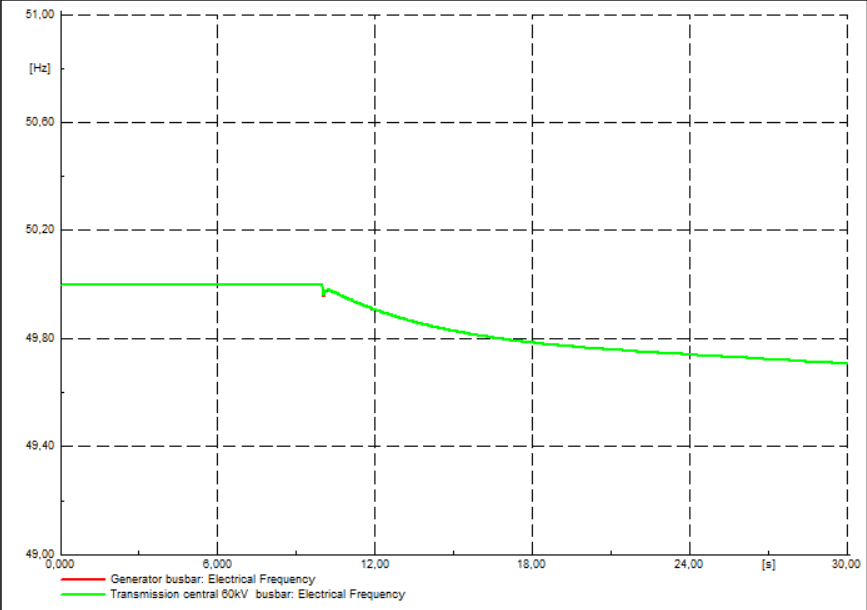
\includegraphics[width=1.00\textwidth]{figurer/LargeDisturbance/Freq2} % Højre billede
	\end{minipage}
	\\ % Figurtekster og labels
	\begin{minipage}[t]{0.48\textwidth}
		\caption{Case 3, Tilstand 2, Spændingsgraf} % Venstre figurtekst og label
		\label{fig:C3T2V}
	\end{minipage}
	\hfill
	\begin{minipage}[t]{0.48\textwidth}
		\caption{Case 3, Tilstand 2, Frekvensgraf} % Højre figurtekst og label
		\label{fig:C3T2F}
	\end{minipage}
\end{figure}

\textbf{Tilstand 3: Alle batterier leverer 1MW med pf 0,95 lagging.}
\begin{figure}[H]
	\centering
	\begin{minipage}[b]{0.48\textwidth}
		\centering
		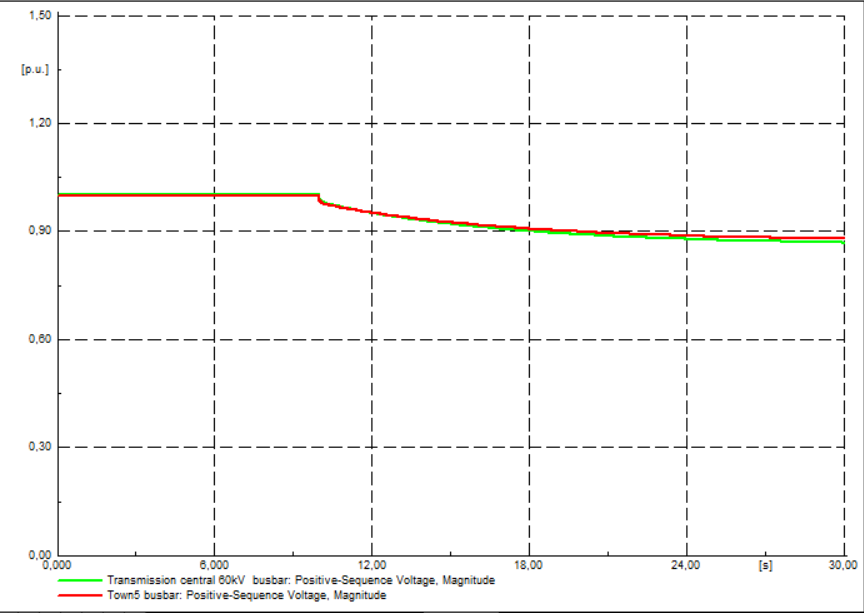
\includegraphics[width=1.00\textwidth]{figurer/LargeDisturbance/Voltage3} % Venstre billede
	\end{minipage}
	\hfill
	\begin{minipage}[b]{0.48\textwidth}
		\centering
		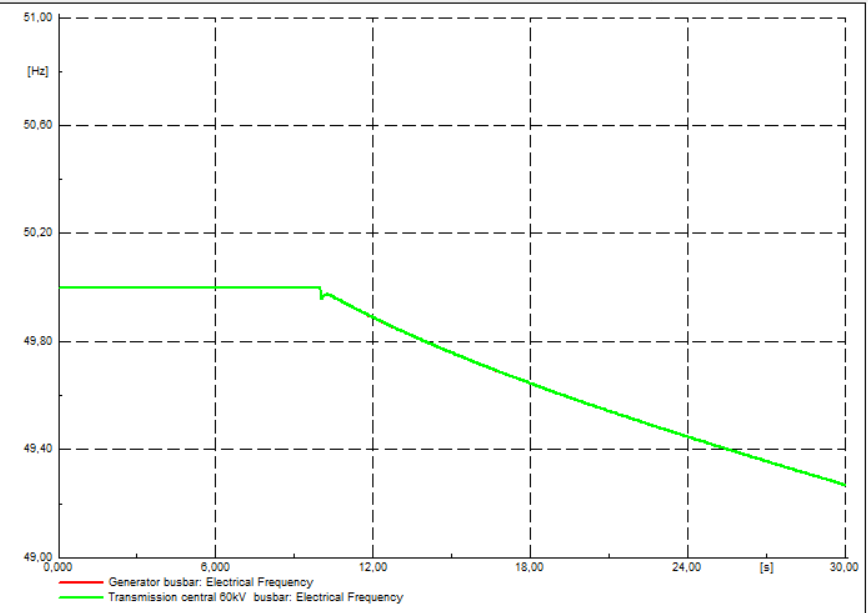
\includegraphics[width=1.00\textwidth]{figurer/LargeDisturbance/Freq3} % Højre billede
	\end{minipage}
	\\ % Figurtekster og labels
	\begin{minipage}[t]{0.48\textwidth}
		\caption{Case 3, Tilstand 3, Spændingsgraf} % Venstre figurtekst og label
		\label{fig:C3T3V}
	\end{minipage}
	\hfill
	\begin{minipage}[t]{0.48\textwidth}
		\caption{Case 3, Tilstand 3, Frekvensgraf} % Højre figurtekst og label
		\label{fig:C3T3F}
	\end{minipage}
\end{figure}

\textbf{Tilstand 4: Alle batterier leverer 1,35MW (Byerne kan betegnes som selvforsynende) med pf 0,95 lagging.}
\begin{figure}[H]
	\centering
	\begin{minipage}[b]{0.48\textwidth}
		\centering
		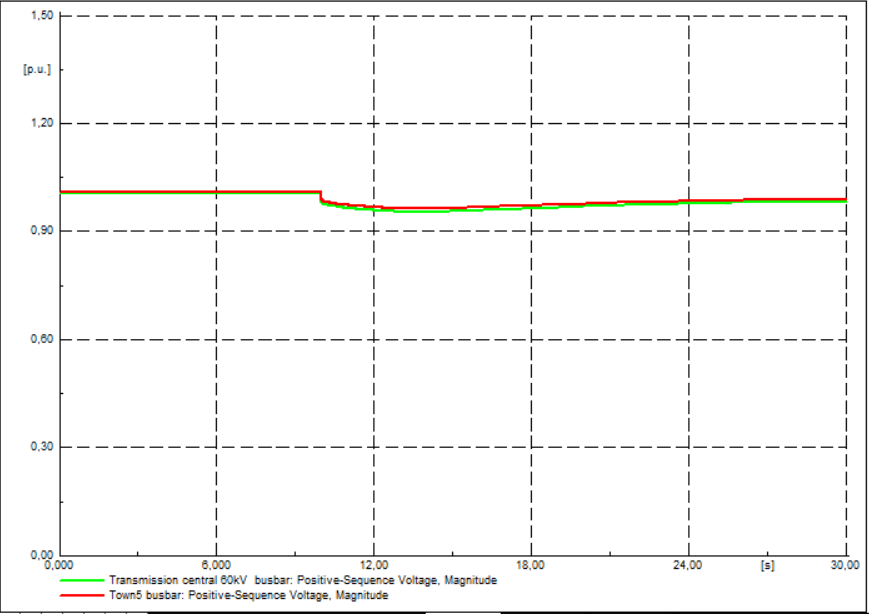
\includegraphics[width=1.00\textwidth]{figurer/LargeDisturbance/Voltage4} % Venstre billede
	\end{minipage}
	\hfill
	\begin{minipage}[b]{0.48\textwidth}
		\centering
		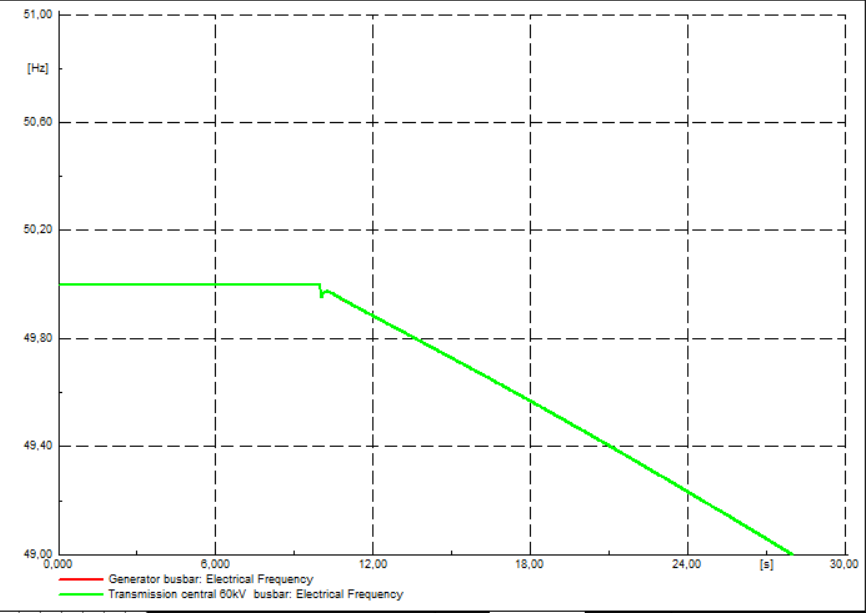
\includegraphics[width=1.00\textwidth]{figurer/LargeDisturbance/Freq4} % Højre billede
	\end{minipage}
	\\ % Figurtekster og labels
	\begin{minipage}[t]{0.48\textwidth}
		\caption{Case 3, Tilstand 4, Spændingsgraf} % Venstre figurtekst og label
		\label{fig:C3T4V}
	\end{minipage}
	\hfill
	\begin{minipage}[t]{0.48\textwidth}
		\caption{Case 3, Tilstand 4, Frekvensgraf} % Højre figurtekst og label
		\label{fig:C3T4F}
	\end{minipage}
\end{figure}

\textbf{Tilstandsoverblik}
\begin{figure}[H] % (alternativt [H])
	\centering
	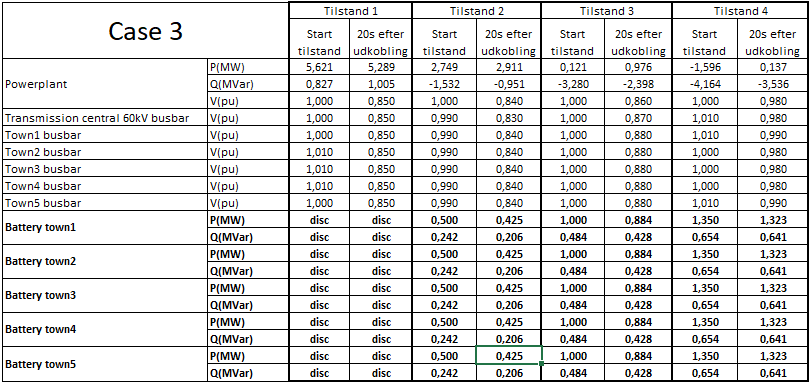
\includegraphics[width=1\textwidth]{figurer/LargeDisturbance/Overview}
	\caption{Overblik for spænding og effektoverførelse i nettet}
	\label{fig:C3Overview}
\end{figure}

Der observeres at når produktionen fra vindmølleparken udkobles vil der opleves et spændingsfald på både \textit{Town5 busbar} - \textit{Town5 busbar} er repræsentativ for alle byer - og \textit{Transmission central 60kV busbar}. Det ses at spændingsfaldet i per unit er af samme størrelsesorden for både \textit{Town5 busbar} og \textit{Transmission central 60kV busbar}. På spændingsgraferne ses det at en stor andel af effektbidrag fra batteri vil resultere i et mindre spændingsfald ved udkobling. Dette skyldes det lavere effektbidrag fra synkron generatoren og derved mindre strøm i transmissions- og distrbutionskabler. I tilstand 4, hvor byerne er selvforsynende - jf. effektbidraget 20s efter udkobling fra Powerpant i tabel \ref{fig:C3Overview} -  ses kun et lille spændingsfald efterfulgt af en spændingsstigning. Spændingen vil stabilisere sig selv efter udkoblingen pga. at produktion og belastning ligger samme sted og der derfor er en meget lille kildeimpedans mellem produktion og belastning.

I forhold til frekvensen observeres det at når andelen af effektbidrag fra batterier øges ses der større fald i frekvensen. Dette tyder på at angående frekvensstabilitet i case 2 er en øget andel forsyning fra husstandsbatterier en ulempe. Grunden til dette er at systemet mister inerti, når synkron generatoren næsten ikke leverer effekt. Synkron generatoren er i dette system kritisk i forhold til inertien, da den er den eneste enhed, der bidrager med inerti. Der observeres i tilstand 1 at frekvensen falder efterfulgt af en frekvensstigning. Dette sker på baggrund af den regulering der er i synkron generatoren, da den vil forsøge at kompensere for tabet af vindmølleparken, imens spændingsfaldet vil resultere en mindre belastning. På et tidspunkt vil produktionen derfor bliver større end forbruget og resultere i en frekvensstigning.
% !TEX root = ../SYSprojektrapport.tex
% SKAL STÅ I TOPPEN AF ALLE FILER FOR AT MASTER-filen KOMPILERES 

\section{Case 4: Den centrale batteriparks evne til at kompensere for tab af produktion}
I dette afsnit præsenteres resultater for simuleringen af case 4 iht. beskrivelsen i afsnit \ref{SimCase1}. I alle fire tilstande er spændingsændringen ved \textit{Town5 busbar} (rød linje) og \textit{Transmission central 60kV busbar} (Grøn linje) samt frekvensændringen på \textit{Transmission central 60kV busbar} (Grøn linje) præsenteret på hhv. spændingsgraf og frekvensgraf. Derudover er der lavet opsamling over spænding samt effektoverførelse andre relevante steder i systemet i tabel \ref{fig:C4Overview}. \\ \\

\textbf{Tilstand 1: Alle batterierne er frakoblet.}
\begin{figure}[H]
	\centering
	\begin{minipage}[b]{0.48\textwidth}
		\centering
		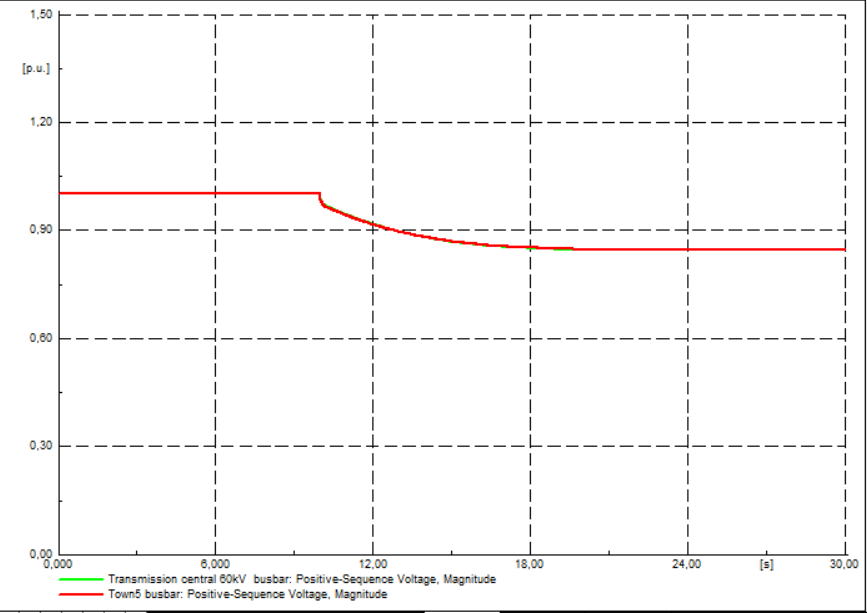
\includegraphics[width=1.00\textwidth]{figurer/LargeDisturbance/Voltage1} % Venstre billede
	\end{minipage}
	\hfill
	\begin{minipage}[b]{0.48\textwidth}
		\centering
		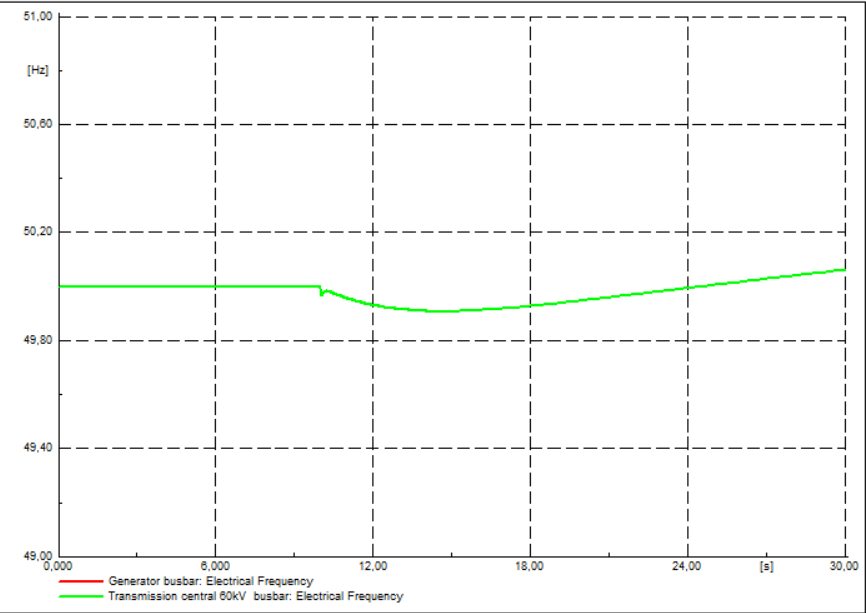
\includegraphics[width=1.00\textwidth]{figurer/LargeDisturbance/Freq1} % Højre billede
	\end{minipage}
	\\ % Figurtekster og labels
	\begin{minipage}[t]{0.48\textwidth}
		\caption{Case 4, Tilstand 1, Spændingsgraf} % Venstre figurtekst og label
		\label{fig:C4T1V}
	\end{minipage}
	\hfill
	\begin{minipage}[t]{0.48\textwidth}
		\caption{Case 4, Tilstand 1, Frekvensgraf} % Højre figurtekst og label
		\label{fig:C4T1F}
	\end{minipage}
\end{figure}

\textbf{Tilstand 2: Batteri central leverer 2,5MW med pf 0,95 lagging.}
\begin{figure}[H]
	\centering
	\begin{minipage}[b]{0.48\textwidth}
		\centering
		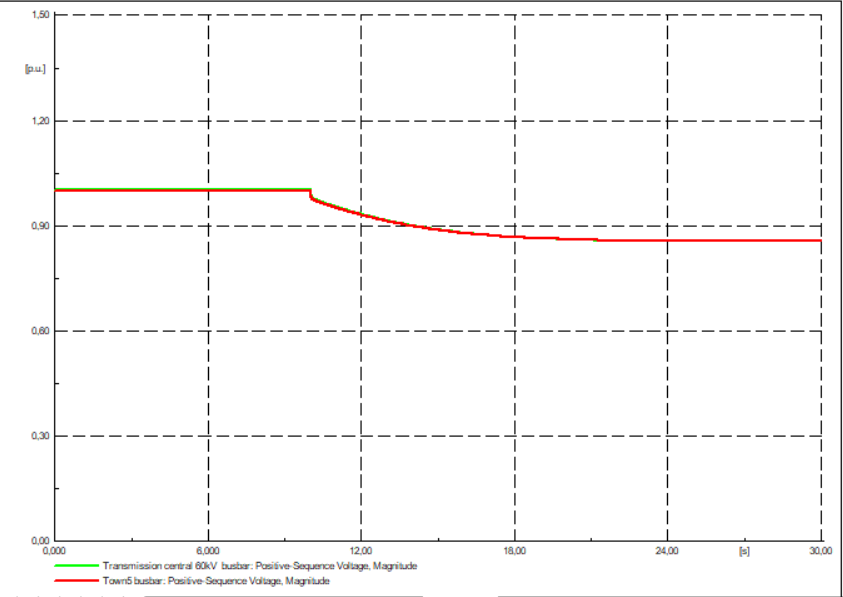
\includegraphics[width=1.00\textwidth]{figurer/LargeDisturbanceBatterypark/Voltage2} % Venstre billede
	\end{minipage}
	\hfill
	\begin{minipage}[b]{0.48\textwidth}
		\centering
		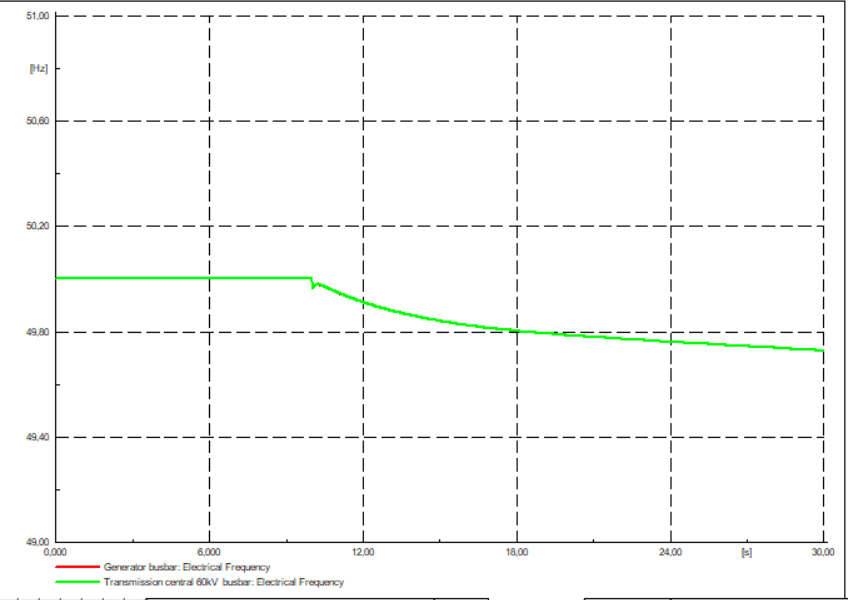
\includegraphics[width=1.00\textwidth]{figurer/LargeDisturbanceBatterypark/Freq2} % Højre billede
	\end{minipage}
	\\ % Figurtekster og labels
	\begin{minipage}[t]{0.48\textwidth}
		\caption{Case 4, Tilstand 2, Spændingsgraf} % Venstre figurtekst og label
		\label{fig:C4T2V}
	\end{minipage}
	\hfill
	\begin{minipage}[t]{0.48\textwidth}
		\caption{Case 4, Tilstand 2, Frekvensgraf} % Højre figurtekst og label
		\label{fig:C4T2F}
	\end{minipage}
\end{figure}

\textbf{Tilstand 3: Batteri central leverer 5MW med pf 0,95 lagging.}
\begin{figure}[H]
	\centering
	\begin{minipage}[b]{0.48\textwidth}
		\centering
		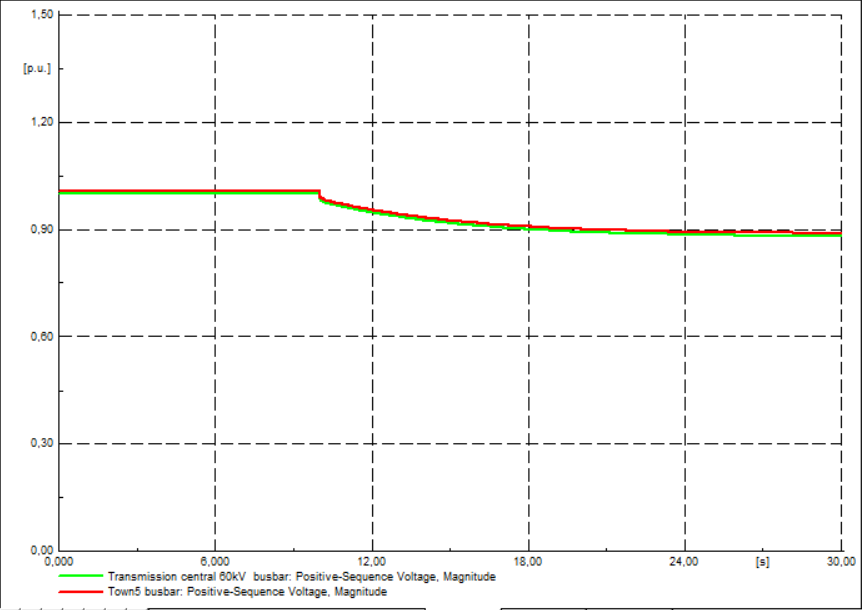
\includegraphics[width=1.00\textwidth]{figurer/LargeDisturbanceBatterypark/Voltage3} % Venstre billede
	\end{minipage}
	\hfill
	\begin{minipage}[b]{0.48\textwidth}
		\centering
		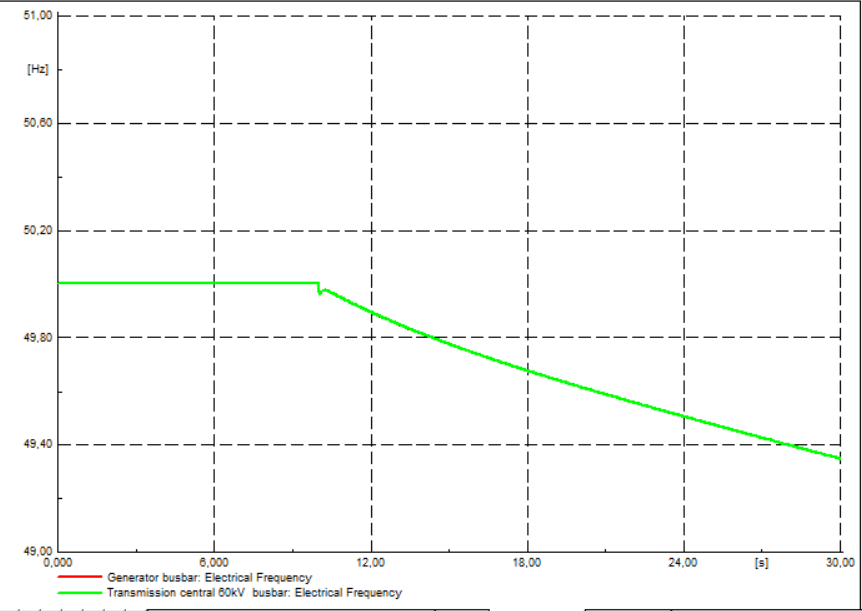
\includegraphics[width=1.00\textwidth]{figurer/LargeDisturbanceBatterypark/Freq3} % Højre billede
	\end{minipage}
	\\ % Figurtekster og labels
	\begin{minipage}[t]{0.48\textwidth}
		\caption{Case 4, Tilstand 3, Spændingsgraf} % Venstre figurtekst og label
		\label{fig:C4T3V}
	\end{minipage}
	\hfill
	\begin{minipage}[t]{0.48\textwidth}
		\caption{Case 4, Tilstand 3, Frekvensgraf} % Højre figurtekst og label
		\label{fig:C4T3F}
	\end{minipage}
\end{figure}

\textbf{Tilstand 4: Batterier leverer 4,41MW med pf 0,95 lagging.}
\begin{figure}[H]
	\centering
	\begin{minipage}[b]{0.48\textwidth}
		\centering
		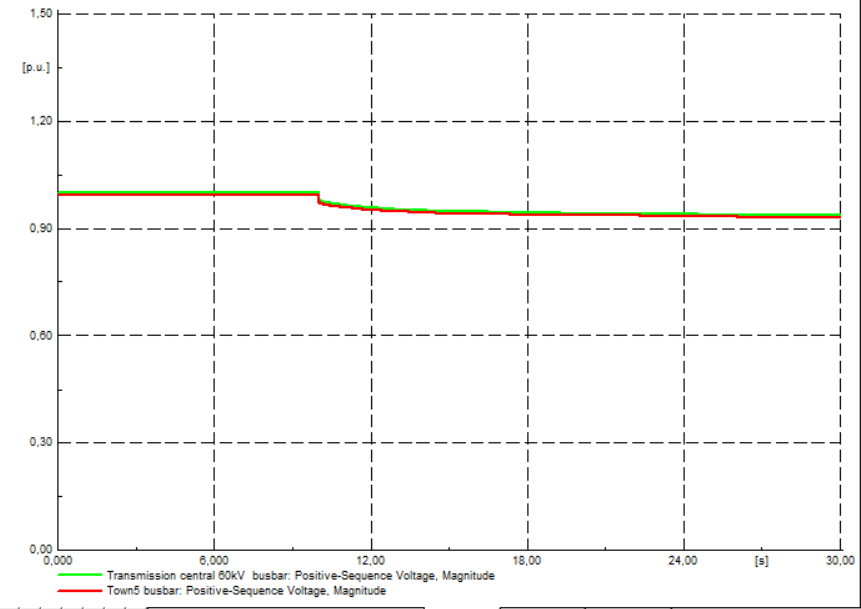
\includegraphics[width=1.00\textwidth]{figurer/LargeDisturbanceBatterypark/Voltage4} % Venstre billede
	\end{minipage}
	\hfill
	\begin{minipage}[b]{0.48\textwidth}
		\centering
		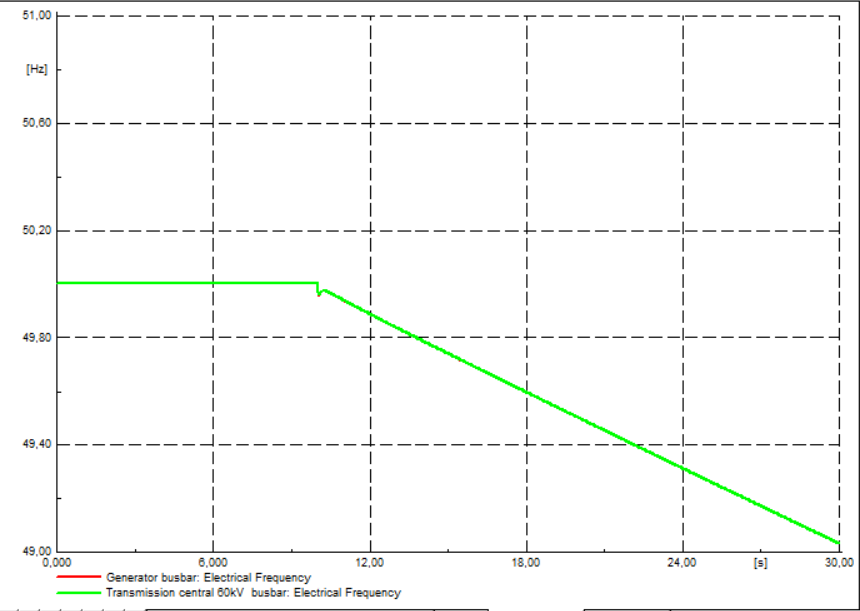
\includegraphics[width=1.00\textwidth]{figurer/LargeDisturbanceBatterypark/Freq4} % Højre billede
	\end{minipage}
	\\ % Figurtekster og labels
	\begin{minipage}[t]{0.48\textwidth}
		\caption{Case 4, Tilstand 4, Spændingsgraf} % Venstre figurtekst og label
		\label{fig:C4T4V}
	\end{minipage}
	\hfill
	\begin{minipage}[t]{0.48\textwidth}
		\caption{Case 4, Tilstand 4, Frekvensgraf} % Højre figurtekst og label
		\label{fig:C4T4F}
	\end{minipage}
\end{figure}

\newpage
\textbf{Tilstandsoverblik}
\begin{figure}[H] % (alternativt [H])
	\centering
	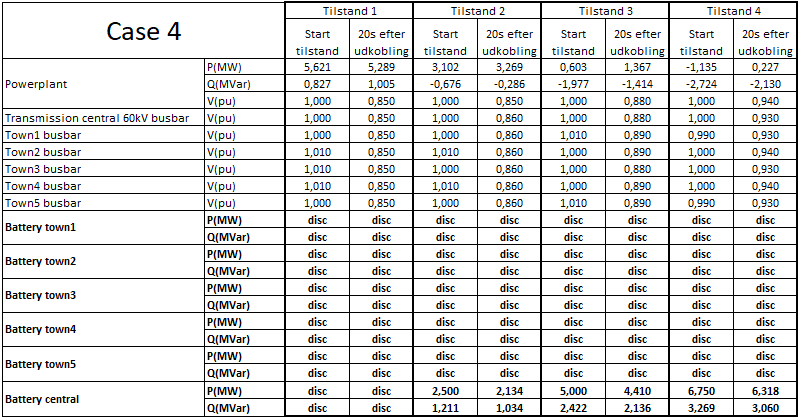
\includegraphics[width=1\textwidth]{figurer/LargeDisturbanceBatterypark/Overview}
	\caption{Overblik for spænding og effektoverførelse i nettet}
	\label{fig:C4Overview}
\end{figure}

I case 4 ses det at tendensen på spændingsgraferne er meget den samme som i case 4. Men ved at sammeholde tilstandsoverblikkene for case 3 og case 4 kan det ses at med en central batteripark, der levere samme effekt som 5 decentrale forsamlinger af batterier, tilsluttet systemet formår nettet at opretholde en højere spænding efter udkoblingen i tilstand 2 og 3. I tilstand 4 ses det at de decentrale batterier kan opretholde den højest spænding. Dette hænger primært sammen med at kildeimpendansen vil være højere i tilfældet med den centrale batteripark, da der er længere ud til belastningen. Det må betyde at de to typer af batteritilslutning har forskellige fordele i forskellige situation. Batteriparkens fordel i tilstand 2 og 3 er i størrelsesorden 0,01-0,03pu, hvilket kan tale for at de decentrale batterier vil være at foretrække, fordi deres fordel i tilstand 4 er noget mere betydelig. Det skal dog bemærkes at i tilstand 4 formår begge typer batterier at opretholde en tilladelig spænding indenfor de $\pm$10\% af nominel spænding.

Angående frekvensen kan der i tilstand 2 ikke observeres en forskel på de to cases. Derimod har den centrale batteripark et mindre frekvensfald i tilstand 3 og 4, hvilket betyder at dette system har den bedste frekvensstabilitet. Dette kan være pga. at den synkrone generator har en større produktion i case 4, der derved giver mere inerti i systemet og gør frekvensen mere stabil. Den ekstra produktion i forhold til case 3, er nødvendig for at kompensere for tabet i kabler og transformere fra den centrale batteripark ud til belastningerne.
\chapter{Konklusion}
% !TEX root = ../prj4projektrapport.tex
% SKAL STÅ I TOPPEN AF ALLE FILER FOR AT MASTER-filen KOMPILERES 

\chapter{Perspektivering}
% !TEX root = ../prj4projektrapport.tex
% SKAL STÅ I TOPPEN AF ALLE FILER FOR AT MASTER-filen KOMPILERES 


\printbibliography

\end{document}


